\documentclass[10pt, letterpaper]{article}

% --- PAQUETES DE IDIOMA Y GRÁFICOS ---
\usepackage[utf8]{inputenc}
\usepackage[T1]{fontenc}
\usepackage[spanish, es-tabla]{babel}
\usepackage{graphicx}
\graphicspath{{imagenes/reporte_tecnico/}{imagenes/}}
\usepackage{tabularx}
\usepackage{booktabs}
\usepackage{amsmath}
\usepackage{amssymb}
\usepackage{amsfonts}

% --- TIPOGRAFÍA TIPO ARIAL ---
% Helvetica es la alternativa más parecida a Arial en LaTeX tradicional
\usepackage[scaled]{helvet}
\renewcommand{\familydefault}{\sfdefault}

% --- DISEÑO Y MÁRGENES ---
\usepackage[
    letterpaper,
    top=20mm,
    bottom=20mm,
    left=25mm,
    right=25mm
]{geometry}

\usepackage{fancyhdr}
\usepackage{float}
\usepackage{xcolor}
\usepackage{colortbl}
\usepackage{parskip}

% --- ESPACIADO ENTRE PÁRRAFOS E INTERLINEADO ---
% El documento pide interlineado de 5.0 pt.
% En LaTeX, esto se aproxima mejor controlando el espacio entre párrafos.
\setlength{\parskip}{5pt}
\setlength{\parindent}{0pt}

% --- COLORES PERSONALIZADOS ---
\definecolor{academicblue}{RGB}{0, 50, 100}

\usepackage[
    colorlinks=true,
    linkcolor=academicblue,
    citecolor=academicblue,
    urlcolor=academicblue
]{hyperref}

% --- ESTILO DE SECCIONES ---
\usepackage{titlesec}

\titleformat{\section}
  {\normalfont\large\bfseries\color{academicblue}}
  {\thesection}{1em}{}

\titleformat{\subsection}
  {\normalfont\normalsize\bfseries\color{academicblue}}
  {\thesubsection}{1em}{}

% Espaciado de secciones para ahorrar espacio
\titlespacing*{\section}{0pt}{10pt}{5pt}
\titlespacing*{\subsection}{0pt}{8pt}{4pt}
\titlespacing*{\paragraph}{0pt}{0pt}{5pt}

% --- ENCABEZADO Y PIE ---
\pagestyle{fancy}
\fancyhf{}
\fancyhead[L]{\small \textit{Gestor de identidades y bases de datos}}
\fancyhead[R]{\small \thepage}
\renewcommand{\headrulewidth}{0.5pt}

\usepackage{longtable}
\usepackage{booktabs}


\begin{document}



% --- PORTADA ---
\begin{titlepage}
    \centering
    
    \vspace{1.5cm}
    
\includegraphics[width=5.5cm]{tecnologico-de-monterrey-blue} 
    
    \vspace{1cm}
    
    {\scshape\LARGE Instituto Tecnológico y de\\Estudios Superiores de Monterrey \par}
    \vspace{0.5cm}
    {\scshape\Large MA2006B.601 - Uso de álgebras modernas para seguridad y criptografía \par}
    
    \vspace{1.5cm}
    
    \hrule height 1.5pt
    \vspace{0.4cm}
    {\huge\bfseries\color{academicblue} Gestor de identidades, registros y bases de datos \par}
    {\Large\bfseries\color{academicblue} Reporte Técnico \par}

    \vspace{0.4cm}
    \hrule height 1.5pt
    
    \vspace{1.5cm}
    
    \begin{center}
    \textbf{Elaborado por:}
    \vspace{1cm}
    
    \begin{tabular}{ll}
        Álvaro Yeudiel Padilla Lobatón & A01665850 \\
        Ricardo Ballesteros Amavizca      & A01255358 \\
        Axel Gabriel Rocha Peréz      & A01067854 \\
        Ana Lidia Arteaga Bretón         & A00838732 \\
        Daniela Ortiz Blanco    & A00840140 \\
        Daniel Garnelo Martínez & A00573086
    \end{tabular}
    \end{center}
    
    \vspace{1.5cm}
    
    \begin{center}
    \large
    \textbf{Profesores:} \\
    Raúl Gómez \;|\; Alberto F. \;|\; Daniel Otero\par
    \vspace{0.2cm}
    \textbf{Fecha:} 14 de junio de 2026
    \end{center}

    \vfill
    \textbf{Casa Monarca Ayuda Humanitaria al Migrante A.B.P.} \\
    \vfill
    {\small Ingeniería en Ciencias de Datos y Matemáticas} \\
    {\small Monterrey, Nuevo León}
\end{titlepage}

\newpage
\tableofcontents
\newpage
\listoffigures
\listoftables
\newpage

\pagestyle{reto_cripto}
\pagenumbering{arabic}

\section{Abstract}

En este proyecto se desarrolló una aplicación web para Casa Monarca orientada a la gestión segura de expedientes de personas atendidas por la organización. La solución busca centralizar la información, proteger los datos sensibles y controlar el acceso de los usuarios mediante diferentes mecanismos de seguridad.

El sistema fue desarrollado en Python utilizando Flask como framework principal y SQLite como base de datos. Para proteger la información se implementó cifrado de expedientes mediante Fernet, autenticación de usuarios con contraseñas protegidas con Argon2id, certificados digitales X.509, passkeys para usuarios con mayores privilegios, control de acceso basado en roles y registros de auditoría. Además, se incorporó un módulo para solicitudes ARCO, con el fin de apoyar el cumplimiento de la Ley General de Protección de Datos Personales.

\section{Introducción}

En la actualidad, muchas organizaciones sociales tienen problemas para manejar información importante, sobre todo cuando todavía dependen de registros en papel o herramientas básicas como formularios en línea. Este es el caso de Casa Monarca, una organización que apoya a personas migrantes y que actualmente no cuenta con un sistema centralizado para gestionar su información.

Esto hace que sea más complicado organizar los datos, tener respaldos confiables y, sobre todo, proteger la información sensible. Al no existir controles claros de acceso, también aumenta el riesgo de que la información se pierda o sea consultada por personas no autorizadas, lo cual es especialmente delicado considerando el tipo de datos que se manejan.

A partir de esto, surge la necesidad de desarrollar una solución que les permita digitalizar y gestionar su información de forma segura, pero también sencilla de usar. La idea es proponer un sistema que no solo organice los datos, sino que también los proteja mediante herramientas de criptografía y control de accesos, adaptándose a las necesidades reales de la organización.

Como resultado se desarrolló una aplicación web funcional para la gestión segura de expedientes en Casa Monarca. La solución integra autenticación mediante usuario y contraseña protegida con Argon2id, autenticación reforzada mediante passkeys y certificados digitales X.509 para usuarios privilegiados, control de acceso basado en roles (RBAC), cifrado de información sensible mediante Fernet, bitácora de auditoría y un módulo para la gestión de solicitudes ARCO. Además, se implementaron mecanismos de protección de sesiones, validación de contraseñas comprometidas y rotación de llaves criptográficas para fortalecer la seguridad general de la plataforma.

\subsection{Relación con los Objetivos de Desarrollo Sostenible}

La solución desarrollada para Casa Monarca contribuye principalmente al Objetivo de Desarrollo Sostenible 16: Paz, Justicia e Instituciones Sólidas, ya que busca fortalecer la protección de información sensible mediante mecanismos de seguridad, autenticación y trazabilidad de acciones dentro del sistema.

Asimismo, contribuye al ODS 10: Reducción de las Desigualdades, al apoyar a una organización que brinda atención a personas migrantes en situación de vulnerabilidad, facilitando una gestión más segura y eficiente de sus expedientes.

\section{Marco de referencia}

Antes de desarrollar la solución tecnológica para Casa Monarca, se analizaron los fundamentos teóricos y las soluciones existentes en la literatura para mitigar los riesgos asociados al manejo de datos sensibles.

\subsection{Seguridad de la información}

Se investigó la tríada de seguridad de la información conocida como CID, la cual constituye uno de los pilares fundamentales para la protección de datos y está compuesta por confidencialidad, integridad y disponibilidad.

La confidencialidad busca garantizar que la información sea accesible únicamente para el personal autorizado. La integridad asegura que los datos no sean alterados, borrados o corrompidos de manera accidental o intencional. Finalmente, la disponibilidad permite que la información esté accesible para los usuarios legítimos cuando la necesiten. Estos tres principios conforman la denominada tríada CID, considerada uno de los fundamentos de la seguridad de la información (Whitman \& Mattord, 2021).

\subsection{Criptografía y cifrado de datos}

La criptografía permite proteger los datos transformándolos para que no sean legibles por personas no autorizadas. Durante el proyecto se revisaron dos tipos principales de criptografía.

La criptografía simétrica utiliza una misma clave para cifrar y descifrar los datos. Este tipo de cifrado es útil para grandes volúmenes de información, ya que suele ser más rápido y eficiente. Por otro lado, la criptografía asimétrica utiliza un par de claves, una pública y una privada, y se usa principalmente en procesos de autenticación, firma digital y protección de claves (Stallings, 2023).

\subsection{Certificados digitales y firmas electrónicas}

Los certificados digitales actúan como credenciales electrónicas que vinculan la identidad de un usuario con una clave pública. Generalmente se utilizan bajo el estándar X.509 y permiten validar que una clave pública pertenece a una persona o entidad específica (Adams \& Lloyd, 2002).

Las firmas digitales permiten comprobar la autenticidad e integridad de una acción o documento. En términos generales, el usuario firma utilizando su clave privada y la verificación se realiza mediante la clave pública correspondiente (Adams \& Lloyd, 2002).

\subsection{Control de accesos}

Para reducir la exposición de la información sensible, se investigó el modelo de Control de Acceso Basado en Roles, conocido como RBAC. Este modelo asigna permisos dependiendo del rol del usuario dentro de la organización, permitiendo limitar las acciones que cada persona puede realizar. Este enfoque es ampliamente utilizado para implementar el principio de mínimo privilegio en sistemas de información (NIST, 2020).

\subsection{Herramientas tecnológicas y entorno de desarrollo}

Para la programación del sistema se utilizó Python, ya que cuenta con librerías enfocadas en seguridad, autenticación y desarrollo web. Entre las herramientas utilizadas se encuentran Flask, SQLite, Cryptography, Fernet, RSA, X.509, WebAuthn, Base64 y Argon2id.

Flask fue utilizado como framework principal para el desarrollo de la aplicación web y la gestión de rutas y sesiones (Pallets Projects, 2024). SQLite se utilizó como base de datos ligera para almacenar usuarios, expedientes, certificados, solicitudes y registros. Fernet se utilizó para el cifrado simétrico de datos sensibles almacenados, mientras que RSA y X.509 se utilizaron para la parte de certificados digitales. WebAuthn permitió integrar passkeys como mecanismo de autenticación reforzada (Python Cryptographic Authority, 2024).

Jinja2 se utilizó para renderizar las plantillas HTML del frontend. Mientras que Requests fue usado para consultas externas como la verificación de contraseñas filtradas. Finalmente, Pytest fue utilizado para pruebas automatizadas del sistema (Python Software Foundation, 2024).

Durante el desarrollo también se analizaron alternativas de infraestructura más robustas, como servicios en la nube. Sin embargo, se buscó priorizar herramientas de bajo costo, fáciles de administrar y acordes a las necesidades actuales de Casa Monarca. De igual forma, se evaluó el uso de llaves físicas de seguridad, aunque son una alternativa segura, implicaban costos y retos logísticos adicionales para la organización, por lo que se optó por passkeys mediante WebAuthn. La Figura \ref{fig:passkey_solucion} muestra el proceso de autenticación reforzada implementado para coordinadores y administradores.

\section{Desarrollo}

\subsection{Propuesta de solución}

Como solución al problema identificado en Casa Monarca, se desarrolló una aplicación web para la gestión segura de expedientes y control de acceso a la información. El objetivo principal fue centralizar el registro y consulta de datos, incorporando mecanismos de seguridad adecuados para proteger la información sensible de las personas atendidas por la organización.

La aplicación fue desarrollada utilizando Flask como framework principal debido a su flexibilidad, facilidad de implementación y amplia disponibilidad de librerías orientadas a seguridad y autenticación. Como sistema de almacenamiento se utilizó SQLite, ya que permite una implementación sencilla sin requerir infraestructura adicional, lo que resulta adecuado para una organización con recursos limitados.

La Figura \ref{fig:login_solucion} muestra la pantalla de inicio de sesión implementada para la plataforma. Desde esta interfaz los usuarios pueden autenticarse utilizando sus credenciales y dependiendo de su rol, continuar con mecanismos adicionales de validación.

\begin{figure}[H]
    \centering
    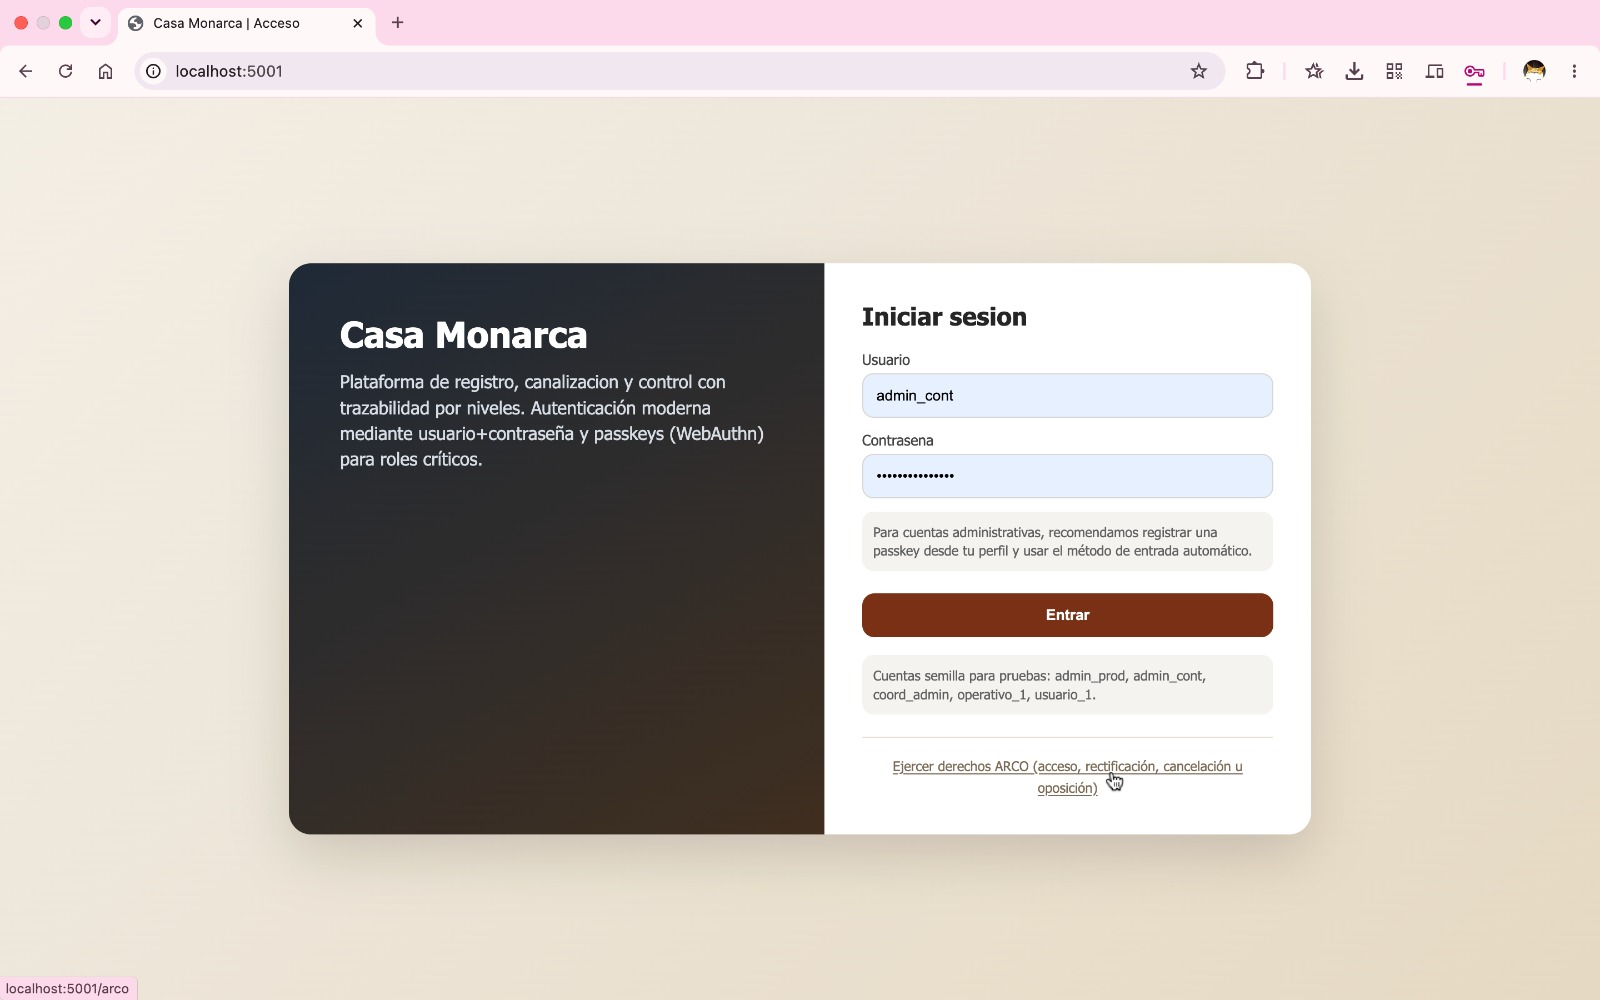
\includegraphics[width=0.8\linewidth]{WhatsApp Image 2026-06-05 at 7.53.43 PM (7).jpeg}
    \caption{Solución - Inicio de Sesión}
    \label{fig:login_solucion}
\end{figure}

Una vez autenticados, acceden al panel principal mostrado en la Figura \ref{fig:panel_admin}. Este es el panel en su vista de administrador, en esta interfaz es posible gestionar usuarios, consultar expedientes, revisar certificados digitales, monitorear registros de auditoría y supervisar las solicitudes realizadas dentro del sistema. Cabe destacar que la plataforma adapta dinámicamente esta vista según los permisos del usuario que inicia sesión (Control de Acceso Basado en Roles) es decir, mientras que la Figura \ref{fig:panel_admin} muestra todas las funciones por ser el nivel con más privilegios, los demás colaboradores visualizarán únicamente las herramientas y módulos estrictamente correspondientes a sus funciones.


\begin{figure} [H]
    \centering
    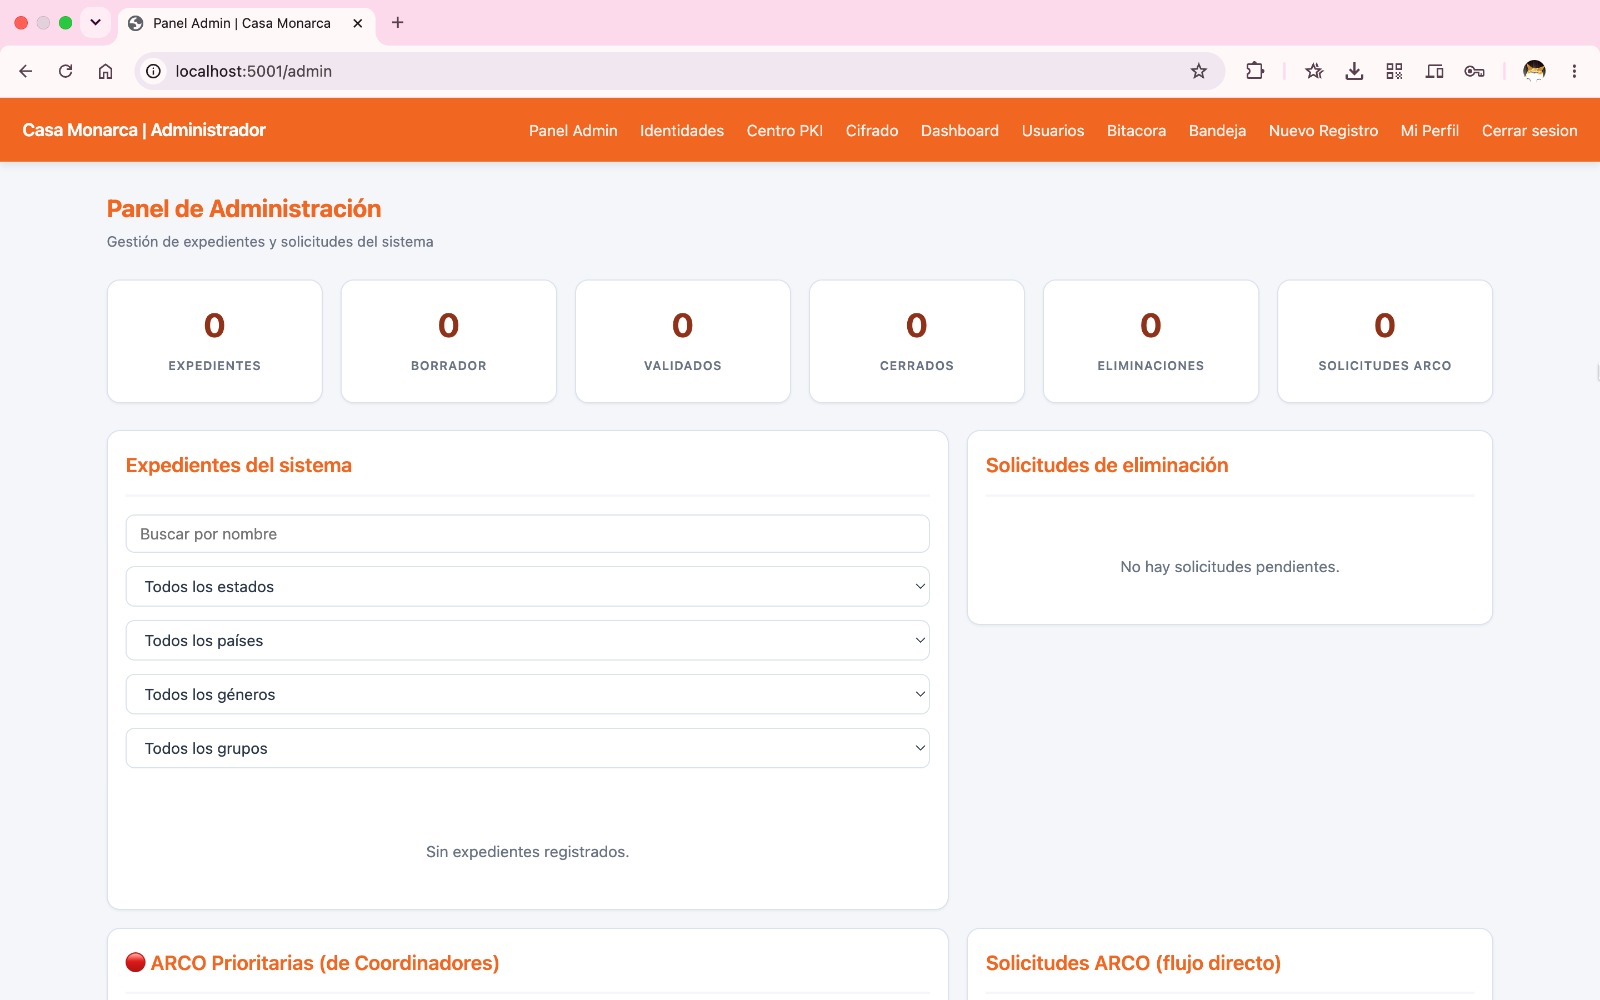
\includegraphics[width=0.8\linewidth]{WhatsApp Image 2026-06-05 at 7.53.43 PM (9).jpeg}
    \caption{Solución - Panel del administrador}
    \label{fig:panel_admin}
\end{figure}

Para reforzar la seguridad se implementaron controles de acceso basados en roles, permitiendo asignar permisos diferentes según las responsabilidades de cada usuario dentro de la organización. Asimismo, se incorporó cifrado de información sensible mediante Fernet, autenticación reforzada mediante certificados digitales X.509 y passkeys para usuarios con privilegios elevados, y un sistema de auditoría encargado de registrar las acciones realizadas dentro de la plataforma.

Como se observa en la Figura \ref{fig:rbac_solucion}, los usuarios se organizan en distintos niveles de acceso, limitando las operaciones que cada uno puede realizar dentro del sistema. En la plataforma, estos niveles van del 1 al 4, diferenciando roles como administradores, coordinadores o voluntarios para establecer qué acciones pueden autorizar, firmar o registrar. Esto permite aplicar el principio de mínimo privilegio y reducir la exposición innecesaria de información sensible.

\begin{figure} [H]
    \centering
    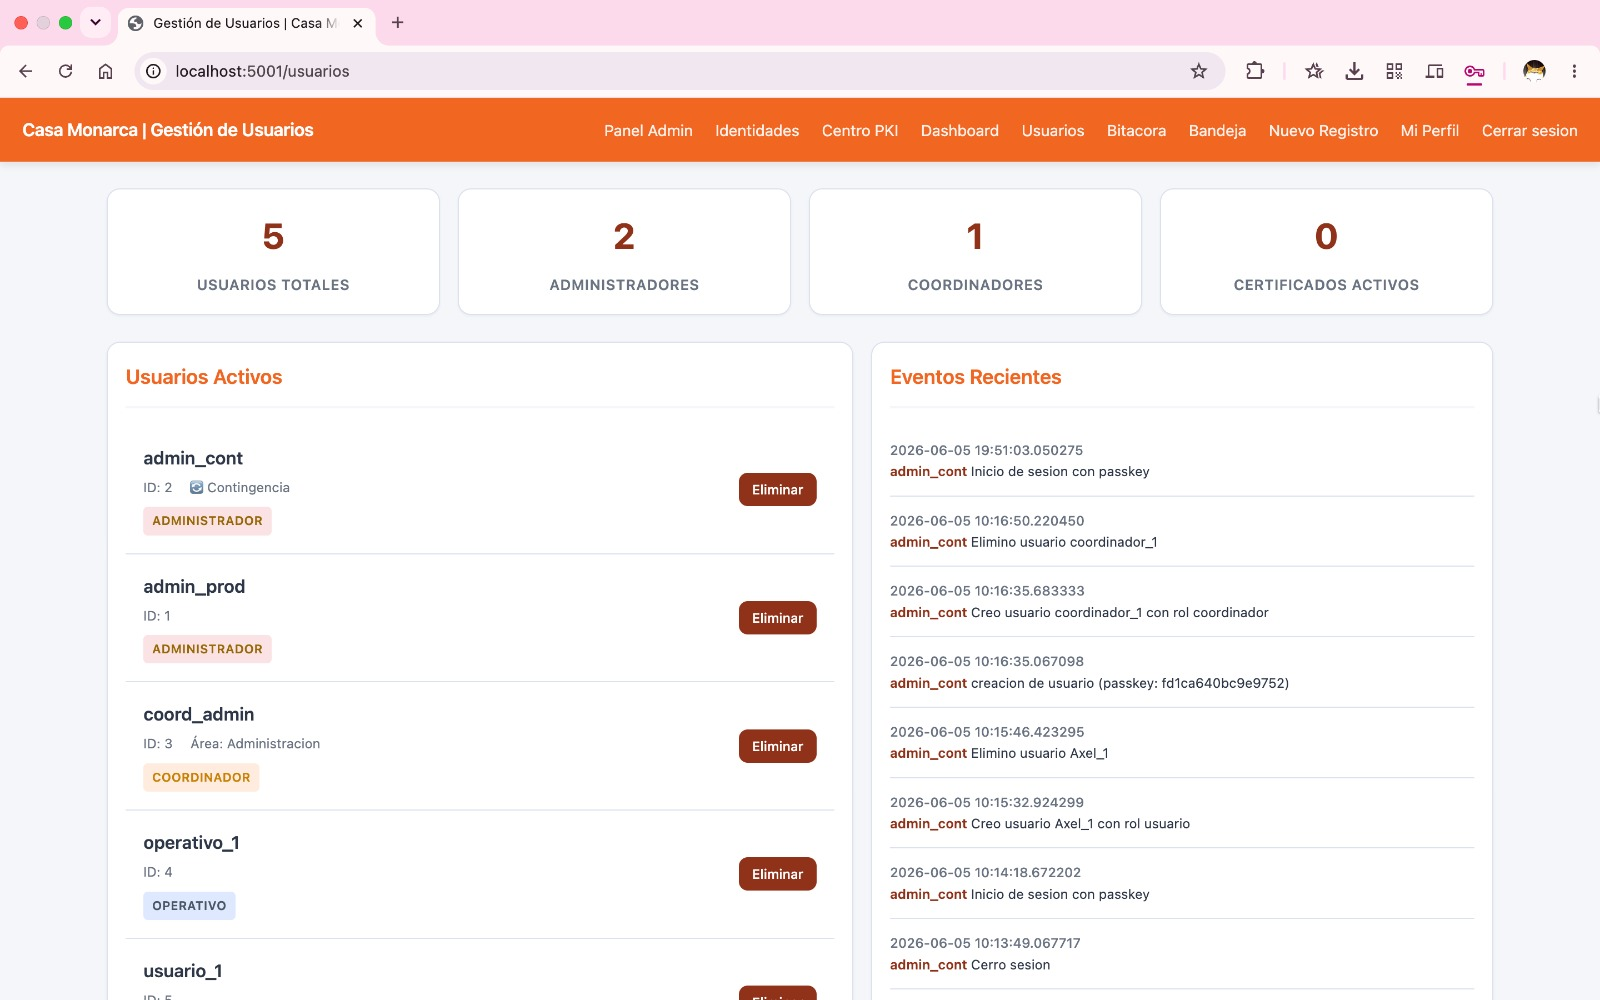
\includegraphics[width=0.8\linewidth]{WhatsApp Image 2026-06-05 at 7.53.43 PM (6).jpeg}
    \caption{Solución - Role Bassed Access Control Y Creación de usuarios.}
    \label{fig:rbac_solucion}
\end{figure}

Adicionalmente, se incorporó un mecanismo de cifrado simétrico para proteger los datos de los expedientes almacenados en la base de datos. La Figura \ref{fig:cifrado_solucion} muestra el módulo utilizado para administrar las claves de encriptación, las cuales tienen tiempos de validez específicos y están reservadas para la vista del administrador.

\begin{figure} [H]
    \centering
    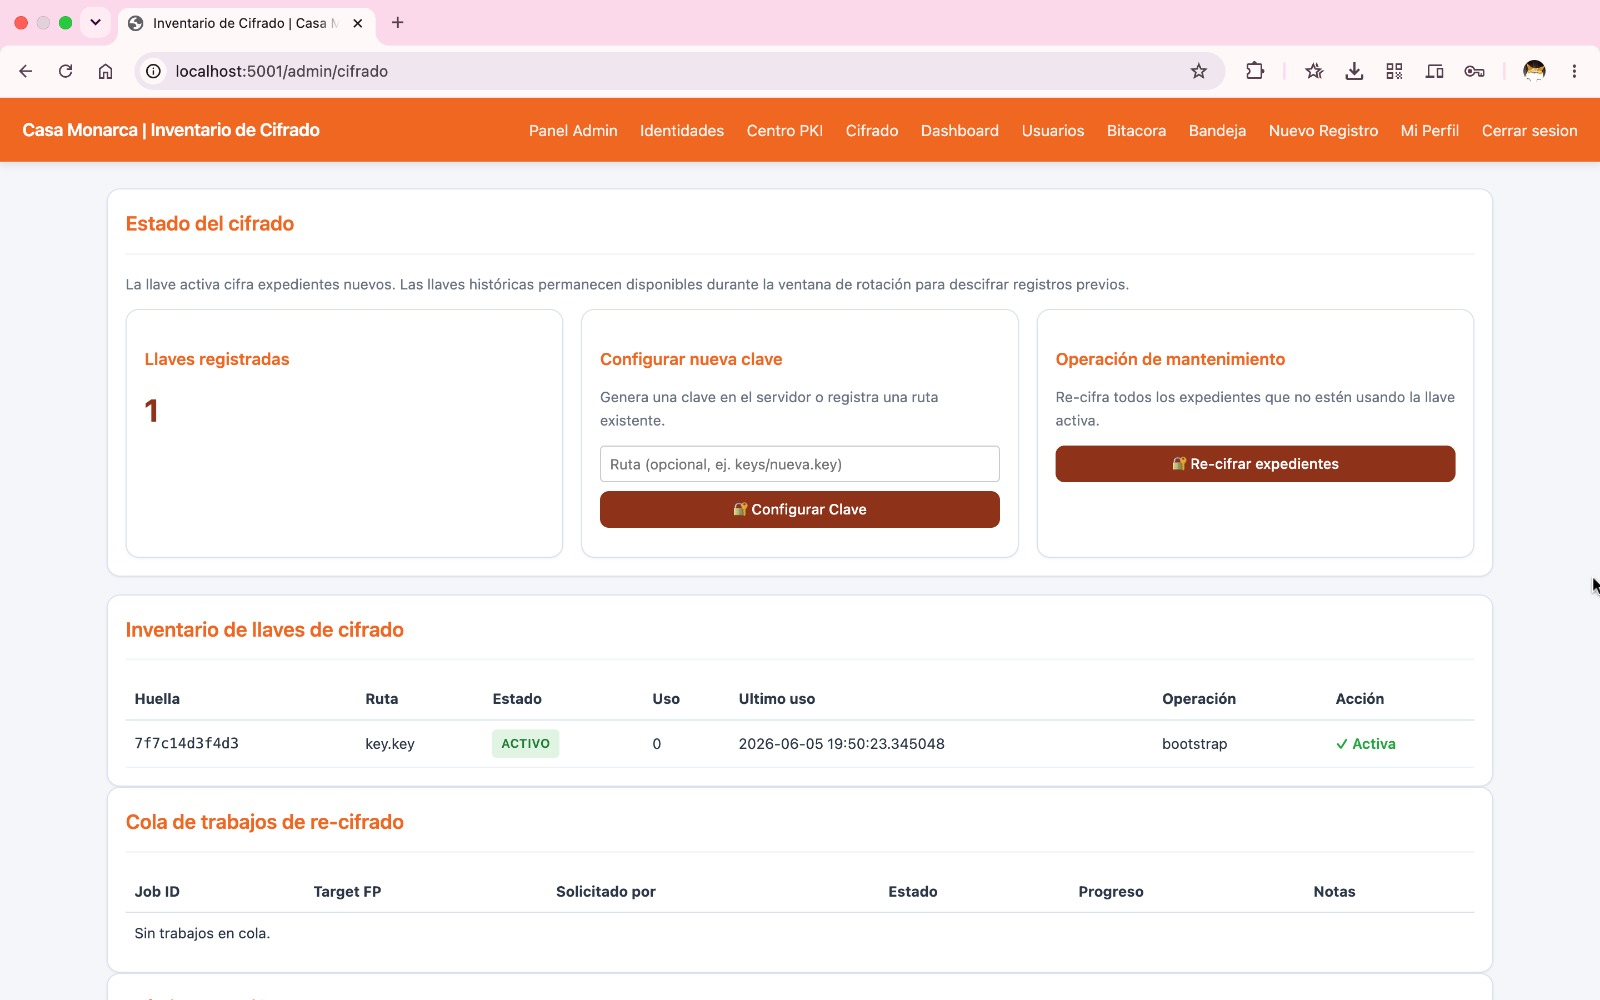
\includegraphics[width=0.8\linewidth]{WhatsApp Image 2026-06-05 at 7.53.43 PM (5).jpeg}
    \caption{Solución - Cifrado de bases de datos.}
    \label{fig:cifrado_solucion}
\end{figure}

Para robustecer la autenticación de los colaboradores, la Figura \ref{fig:passkey_solucion} ilustra la integración de Passkeys (WebAuthn). Esto permite un inicio de sesión seguro mediante factores locales como la huella dactilar, garantizando que el contenido de las claves no se libere ni quede expuesto. 

\begin{figure} [H]
    \centering
    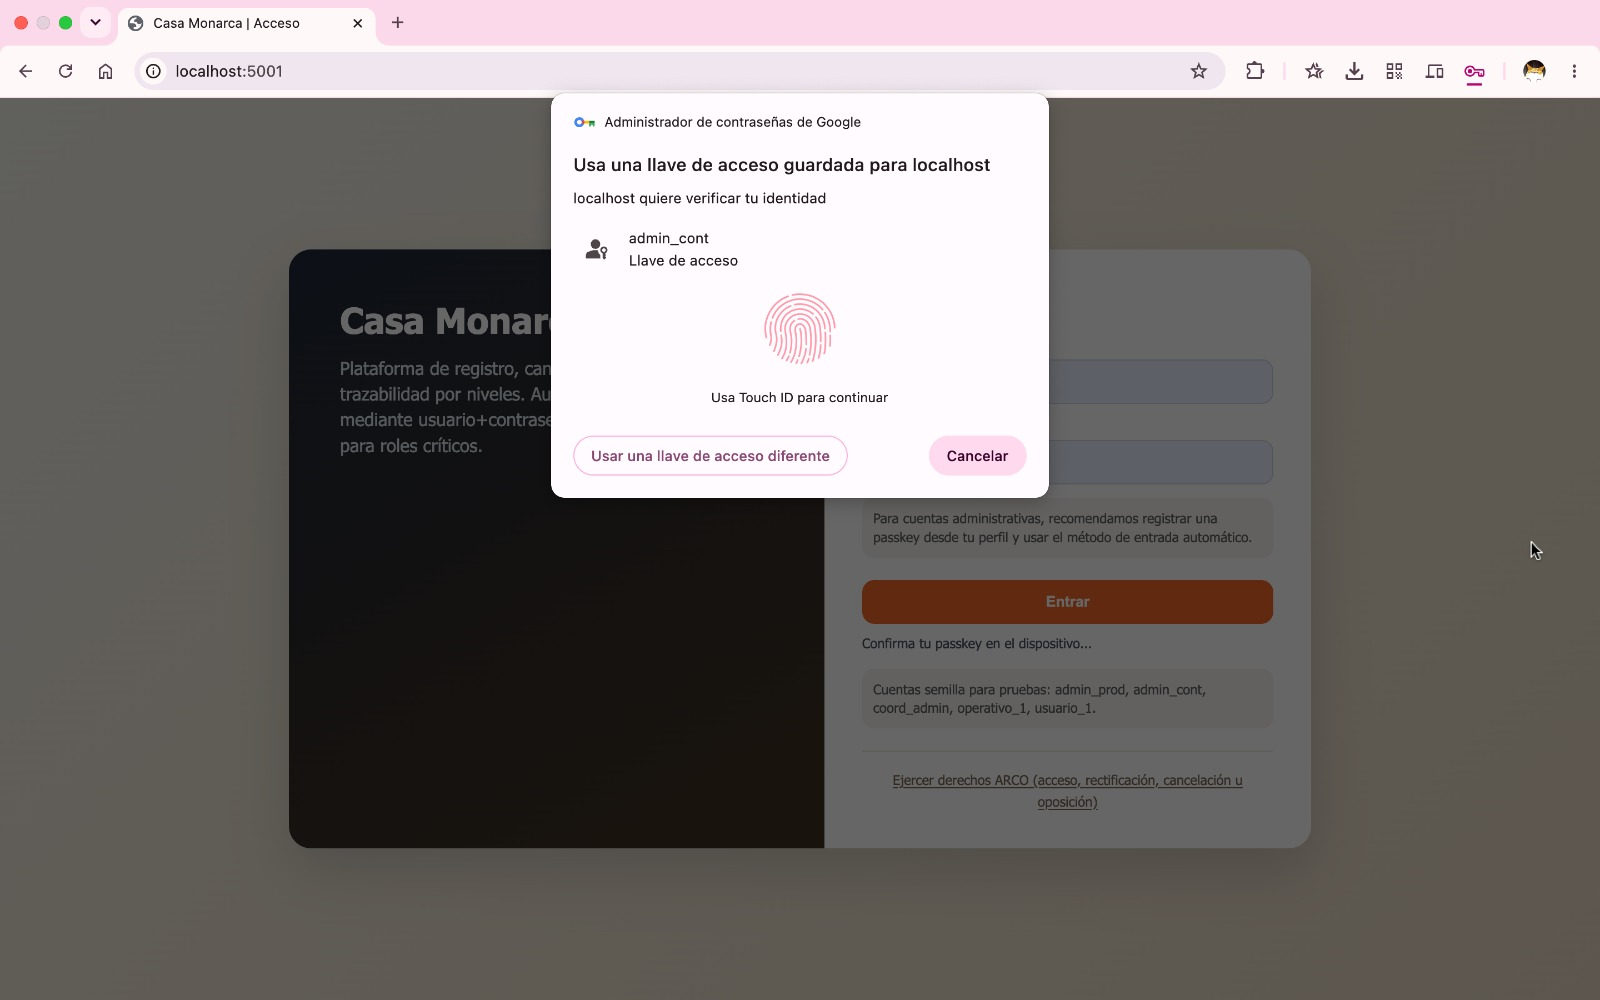
\includegraphics[width=0.8\linewidth]{WhatsApp Image 2026-06-05 at 7.53.43 PM (4).jpeg}
    \caption{Solución - Passkey en inicio de sesión.}
    \label{fig:passkey_solucion}
\end{figure}

Adicionalmente, el sistema incorpora mecanismos orientados al cumplimiento de la Ley General de Protección de Datos Personales (LGDP) mediante la gestión de solicitudes ARCO (Acceso, Rectificación, Cancelación y Oposición). La interfaz desarrollada para este proceso se muestra en la Figura \ref{fig:arco_solucion}, permitiendo registrar y dar seguimiento a solicitudes relacionadas con acceso, rectificación, cancelación u oposición de datos personales.

\begin{figure} [H]
    \centering
    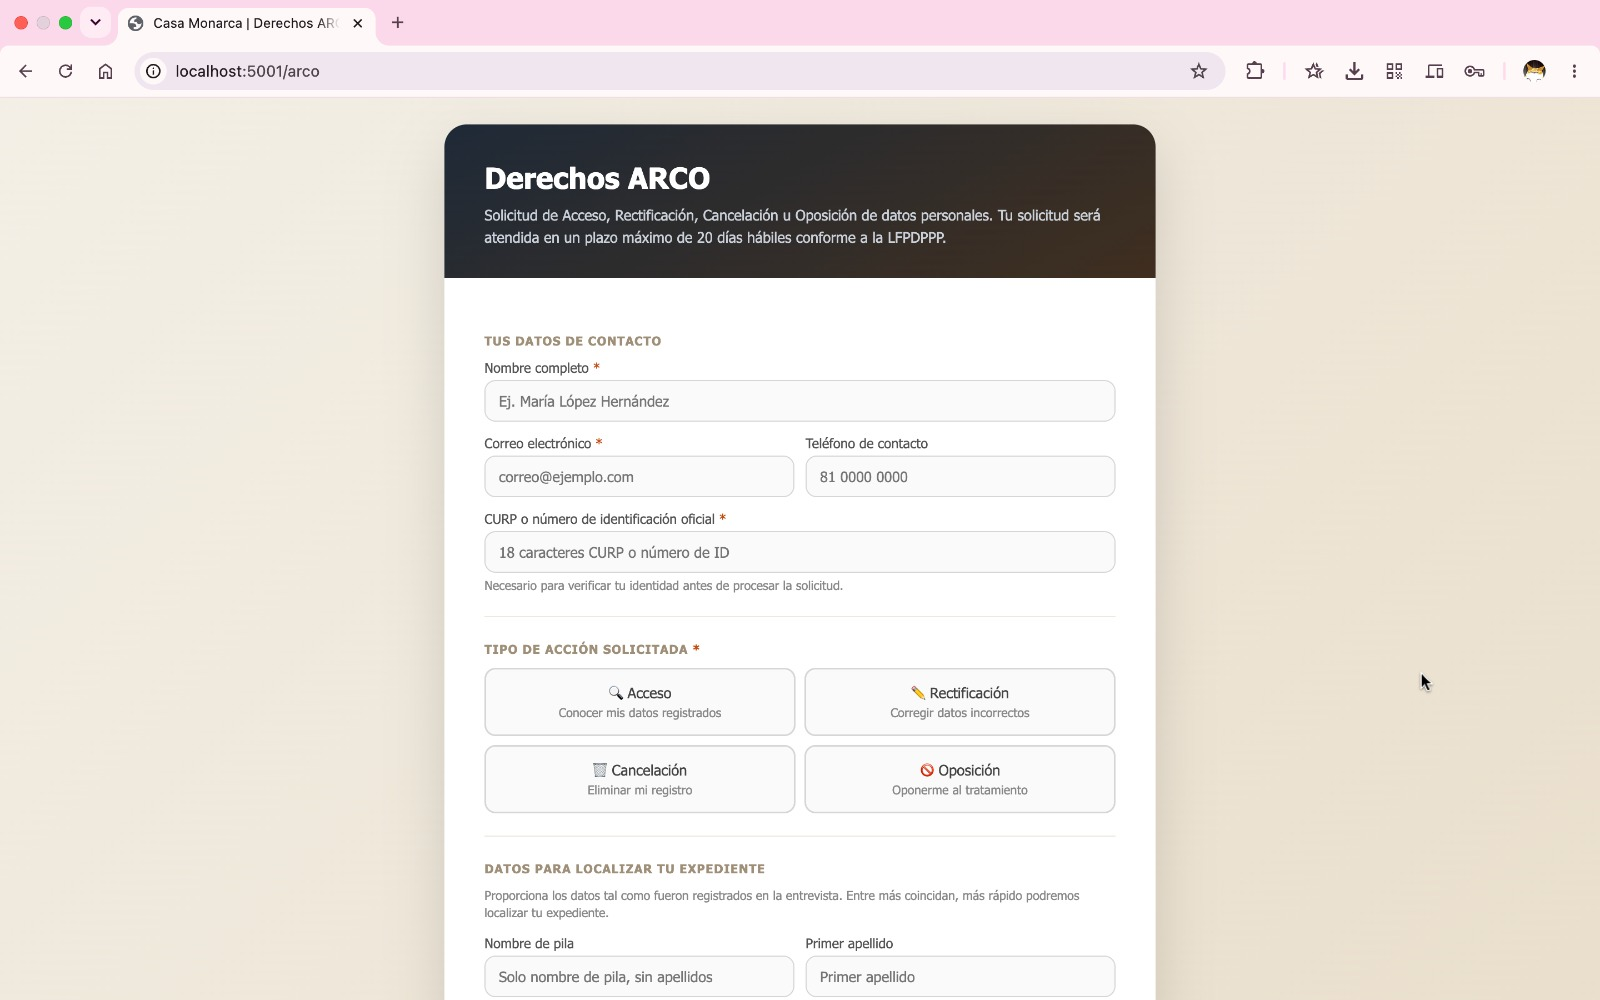
\includegraphics[width=0.8\linewidth]{WhatsApp Image 2026-06-05 at 7.53.43 PM.jpeg}
    \caption{Solución - Sección de los derechos ARCO}
    \label{fig:arco_solucion}
\end{figure}

\subsection{Desarrollo del Backend}

El backend de la aplicación fue desarrollado en Python utilizando Flask. Esta parte del sistema es la encargada de procesar la lógica principal de la plataforma, validar usuarios, controlar permisos, proteger la información almacenada y registrar las acciones realizadas dentro del sistema.

\subsubsection{Gestión de usuarios y roles}

Para la gestión de usuarios y roles se implementaron distintos tipos de usuario dentro del sistema: usuario básico, operativo, coordinador y administrador. Cada uno de estos roles cuenta con permisos diferentes, de acuerdo con las funciones que puede realizar dentro de la plataforma.

El sistema utiliza un modelo de control de acceso basado en roles, conocido como RBAC. Este modelo permite definir qué acciones puede realizar cada usuario, organizando los permisos principales en crear, leer, actualizar y eliminar información. Estos permisos aumentan de acuerdo con el nivel del rol; por ejemplo, el usuario básico puede crear registros, el operativo puede crear y leer, el coordinador puede crear, leer y actualizar, mientras que el administrador cuenta con permisos completos.

Además de los permisos generales, el backend también controla el avance de los expedientes según el rol del usuario. Esto evita que una sola persona pueda modificar todo el proceso por sí misma, ya que ciertas etapas deben ser revisadas o validadas por un coordinador o administrador.

\subsubsection{Sistema de autenticación}

La plataforma tiene un sistema de autenticación basado en usuario y contraseña para todos los usuarios. Para proteger las credenciales se utilizó Argon2id, un algoritmo especializado para el almacenamiento seguro de contraseñas. Adicionalmente, se emplea un salt aleatorio para evitar que dos usuarios con la misma contraseña generen hashes idénticos.

También se implementó un mecanismo de bloqueo temporal después de varios intentos fallidos de inicio de sesión. Esto permite reducir el riesgo de ataques de fuerza bruta y proteger las cuentas frente a accesos no autorizados.

Además, se agrego una validación de contraseñas mínimas, verificación contra contraseñas comunes o comprometidas y protección CSRF (Cross-Site Request Forgery) en formularios.

Adicionalmente, el sistema contempla la existencia de cuentas de contingencia destinadas a escenarios de recuperación operativa. Estas cuentas permiten mantener la administración de la plataforma en caso de pérdida de credenciales, expiración de certificados o fallos en mecanismos de autenticación avanzados. Su uso se encuentra restringido a personal autorizado y debe registrarse dentro de la bitácora de auditoría para mantener la trazabilidad de las acciones realizadas.

\subsubsection{Protección de sesiones y formularios}

Además de la autenticación, el sistema incorpora mecanismos de protección para las sesiones y formularios utilizados por los usuarios. Entre ellos se encuentra la protección CSRF (Cross-Site Request Forgery), la cual agrega tokens de validación a los formularios para verificar que las solicitudes realmente provienen de la aplicación y no de sitios externos maliciosos.

Asimismo, se configuraron las cookies de sesión utilizando atributos de seguridad como \textit{HttpOnly} y \textit{SameSite}. El atributo \textit{HttpOnly} impide que scripts ejecutados desde el navegador puedan acceder directamente a la cookie de sesión, reduciendo el riesgo de robo de credenciales mediante ataques de tipo Cross-Site Scripting (XSS). Por su parte, \textit{SameSite} limita el envío automático de cookies cuando las solicitudes provienen de otros sitios web, ayudando a prevenir ataques de suplantación de solicitudes.

\subsubsection{Certificados digitales y passkeys}

Para los coordinadores y administradores se implementó una capa adicional de seguridad mediante certificados digitales X.509 y passkeys. Estos mecanismos utilizan criptografía asimétrica para verificar la identidad del usuario sin necesidad de compartir información sensible.

Las passkeys funcionan mediante un esquema de challenge-response, donde el servidor genera un desafío que es firmado utilizando una clave privada protegida por el dispositivo del usuario. Posteriormente, el sistema verifica la firma utilizando la clave pública registrada, permitiendo confirmar la identidad del usuario de forma segura.

Además, las acciones sensibles pueden requerir una firma adicional con passkey, la cual se valida por un periodo corto y se consume después de utilizarse.

\subsubsection{Cifrado y protección de datos}

La información sensible almacenada en los expedientes es cifrada antes de guardarse en la base de datos mediante Fernet. Esto permite proteger los datos frente a accesos no autorizados y proteger los datos almacenados en reposo. El acceso a la información se controla mediante el modelo de permisos del sistema.

Además, se incorporó un sistema de administración y rotación de llaves que facilita la gestión del cifrado a lo largo del tiempo, permitiendo mantener la protección de la información conforme evoluciona el sistema.

\subsubsection{Auditoría y trazabilidad}

El sistema incorpora una bitácora de auditoría encargada de registrar eventos relevantes, tales como inicios de sesión, creación de usuarios, modificaciones de expedientes, uso de certificados y acciones administrativas.

Estos registros permiten mantener trazabilidad sobre las operaciones realizadas dentro de la plataforma, facilitando la identificación de accesos indebidos o cambios realizados sobre la información.

También se registran métricas relacionadas con operaciones de cifrado y descifrado, como la llave utilizada y el tiempo de operación. Un ejemplo de los registros almacenados por el sistema puede observarse en la Figura \ref{fig:bitacora_solucion}, donde se muestran eventos asociados a la actividad de los usuarios dentro de la plataforma.

\begin{figure} [H]
    \centering
    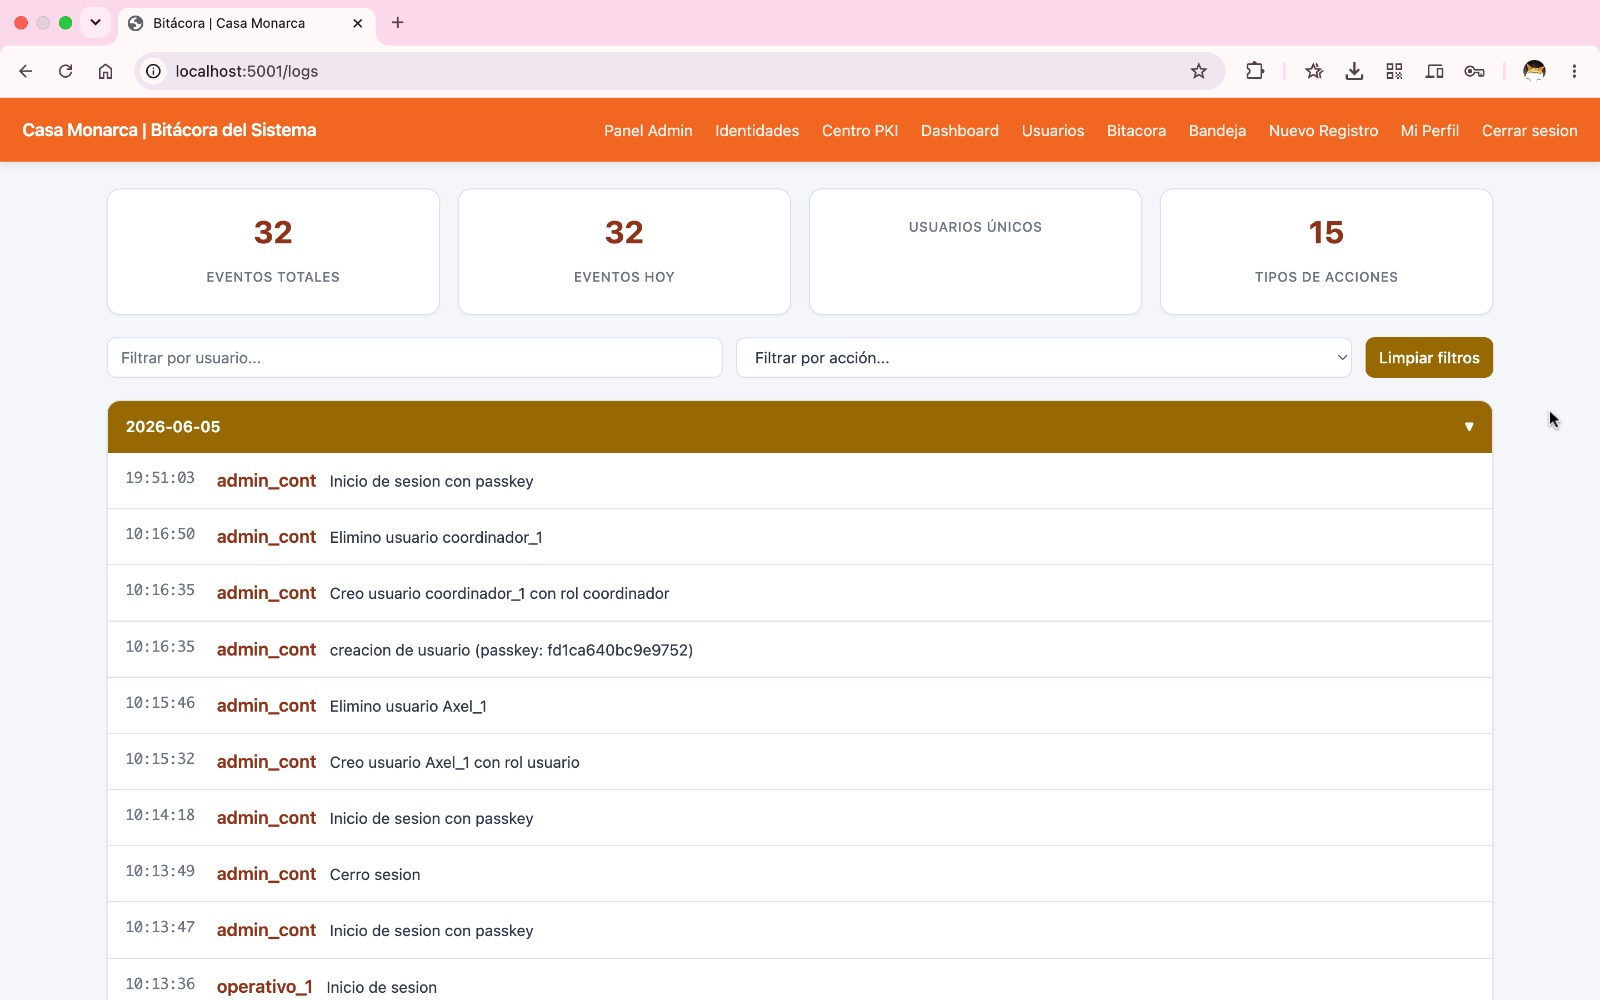
\includegraphics[width=0.8\linewidth]{WhatsApp Image 2026-06-05 at 7.53.43 PM (8).jpeg}
    \caption{Solución - Bitácora}
    \label{fig:bitacora_solucion}
\end{figure}

\subsubsection{Gestión de solicitudes ARCO}

Como parte del cumplimiento de la Ley General de Protección de Datos Personales, se desarrolló un módulo para la gestión de solicitudes ARCO, relacionadas con los derechos de Acceso, Rectificación, Cancelación y Oposición establecidos en la Ley Federal de Protección de Datos Personales en Posesión de los Particulares (Cámara de Diputados del H. Congreso de la Unión, 2017).

Este módulo permite que las solicitudes sean registradas y evaluadas mediante un flujo de revisión que involucra a los distintos niveles de la organización, garantizando un tratamiento controlado de la información personal.

\subsection{Desarrollo del Frontend}

El frontend de la aplicación fue desarrollado como una interfaz web que permite a los usuarios interactuar con el sistema de forma sencilla. Su objetivo principal es facilitar el acceso a las distintas funcionalidades de la plataforma, manteniendo una experiencia de uso adecuada para los diferentes perfiles de usuario.

Se desarrollaron pantallas para el inicio de sesión, registro y consulta de expedientes, administración de usuarios, gestión de certificados y seguimiento de solicitudes ARCO. La información mostrada en cada sección depende del rol del usuario autenticado, permitiendo que cada persona visualice únicamente las funciones que le corresponden.

Además, se incorporaron formularios para la captura de información, validaciones básicas de entrada y mecanismos de protección asociados a la sesión del usuario. Esto permite reducir errores durante el uso de la plataforma y mantener una interacción más segura con el sistema.

\subsection{Arquitectura del sistema}

La arquitectura del sistema se ha diseñado bajo un enfoque modular, estructurado en capas que garantizan la separación de responsabilidades y la integridad de los datos. En la Figura \ref{fig:arquitectura} se muestra la organización lógica de los componentes que integran la plataforma, detallando la interacción entre las capas de presentación, lógica de negocio, cifrado y persistencia de datos.

\begin{figure} [H]
    \centering
    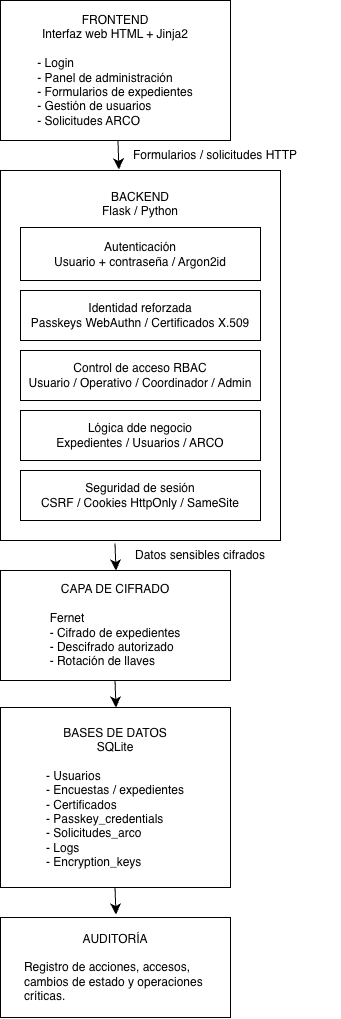
\includegraphics[width=0.4\linewidth]{Cripto.drawio.png}
    \caption{Arquitectura lógica de los componentes del sistema.}
    \label{fig:arquitectura}
\end{figure}

Para garantizar el cumplimiento de los protocolos de seguridad definidos, el sistema sigue un flujo procedimental estricto que evalúa la identidad y los privilegios del usuario. Como se observa en la Figura \ref{fig:arquitectura2}, el proceso de autenticación y acceso evidencia las decisiones de seguridad, las validaciones multifactor (MFA) y la aplicación del control de acceso basado en roles (RBAC) antes de permitir la interacción con los módulos del sistema.

\begin{figure} [H]
    \centering
    \includegraphics[width=0.45\linewidth]{Cripto-Copia de Página-1.drawio.png}
    \caption{Diagrama de flujo del proceso de autenticación y acceso.}
    \label{fig:arquitectura2}
\end{figure}

\subsection{Conexión de componentes}

La solución fue diseñada para integrar los distintos componentes de manera centralizada. El frontend se comunica con el backend mediante las rutas definidas en Flask, permitiendo enviar solicitudes y recibir la información correspondiente.

Cuando un usuario realiza una acción, el backend verifica primero sus permisos y posteriormente procesa la solicitud. En caso de tratarse de información sensible, los datos son cifrados antes de almacenarse en la base de datos. Del mismo modo, cuando la información es consultada, el sistema valida los permisos del usuario antes de mostrar el contenido correspondiente.

Adicionalmente, los procesos de autenticación, certificados digitales, passkeys, auditoría y solicitudes ARCO se encuentran integrados dentro del mismo flujo de trabajo, permitiendo que los distintos mecanismos de seguridad funcionen de forma conjunta.

En el caso de las passkeys, el frontend solicita al navegador la firma de un reto criptográfico generado por el backend. Posteriormente, la respuesta firmada es enviada nuevamente al servidor, donde se valida utilizando la clave pública previamente registrada para el usuario. Este proceso permite autenticar la identidad del usuario sin transmitir claves privadas ni contraseñas adicionales a través de la red.

\section{Resultados}

Como resultado del proyecto se obtuvo una aplicación funcional capaz de gestionar expedientes de manera centralizada e incorporar mecanismos de seguridad orientados a la protección de información sensible.

\subsection{Resultados del Backend}

Se logró implementar un sistema de gestión de usuarios con distintos niveles de acceso, autenticación mediante contraseñas protegidas con Argon2id, autenticación reforzada mediante certificados digitales y passkeys, cifrado de expedientes mediante Fernet y un sistema de auditoría para el registro de actividades. Asimismo, se desarrolló un módulo para la gestión de solicitudes ARCO, permitiendo apoyar el cumplimiento de los lineamientos relacionados con la protección de datos personales.

Como evidencia del funcionamiento del backend, la Figura \ref{fig:bitacora_solucion} muestra registros generados automáticamente por el sistema durante distintas operaciones. Estos registros permiten verificar el correcto funcionamiento de los mecanismos de auditoría y trazabilidad implementados.

\subsection{Resultados del Frontend}

Se desarrollaron interfaces para la administración de usuarios, captura y consulta de expedientes, autenticación, visualización de registros y gestión de solicitudes ARCO. Estas interfaces permitieron validar el funcionamiento de los distintos módulos del sistema, incluyendo la gestión de certificados, la consulta de bitácoras y los mecanismos de control de acceso. Además, la información mostrada se adapta dinámicamente al rol del usuario, garantizando que cada perfil acceda únicamente a las funcionalidades que tiene autorizadas.

\subsection{Resultados de la solución completa}

La integración de todos los componentes permitió construir una plataforma capaz de centralizar la información de Casa Monarca, controlar el acceso a los datos y mantener un registro de las acciones realizadas dentro del sistema. Las pruebas realizadas demostraron el correcto funcionamiento de los mecanismos de autenticación, cifrado, control de acceso y auditoría implementados durante el desarrollo.

\subsection{Casos de uso y validaciones}

\begin{center}
\renewcommand{\arraystretch}{2.5}

\begin{longtable}{p{0.22\linewidth} p{0.10\linewidth} p{0.53\linewidth}}

\toprule
\textbf{Caso de prueba} & \textbf{Resultado} & \textbf{Evidencia} \\
\midrule
\endfirsthead

\toprule
\textbf{Caso de prueba} & \textbf{Resultado} & \textbf{Evidencia} \\
\midrule
\endhead

Inicio de sesión con usuario y contraseña
&
Correcto
&
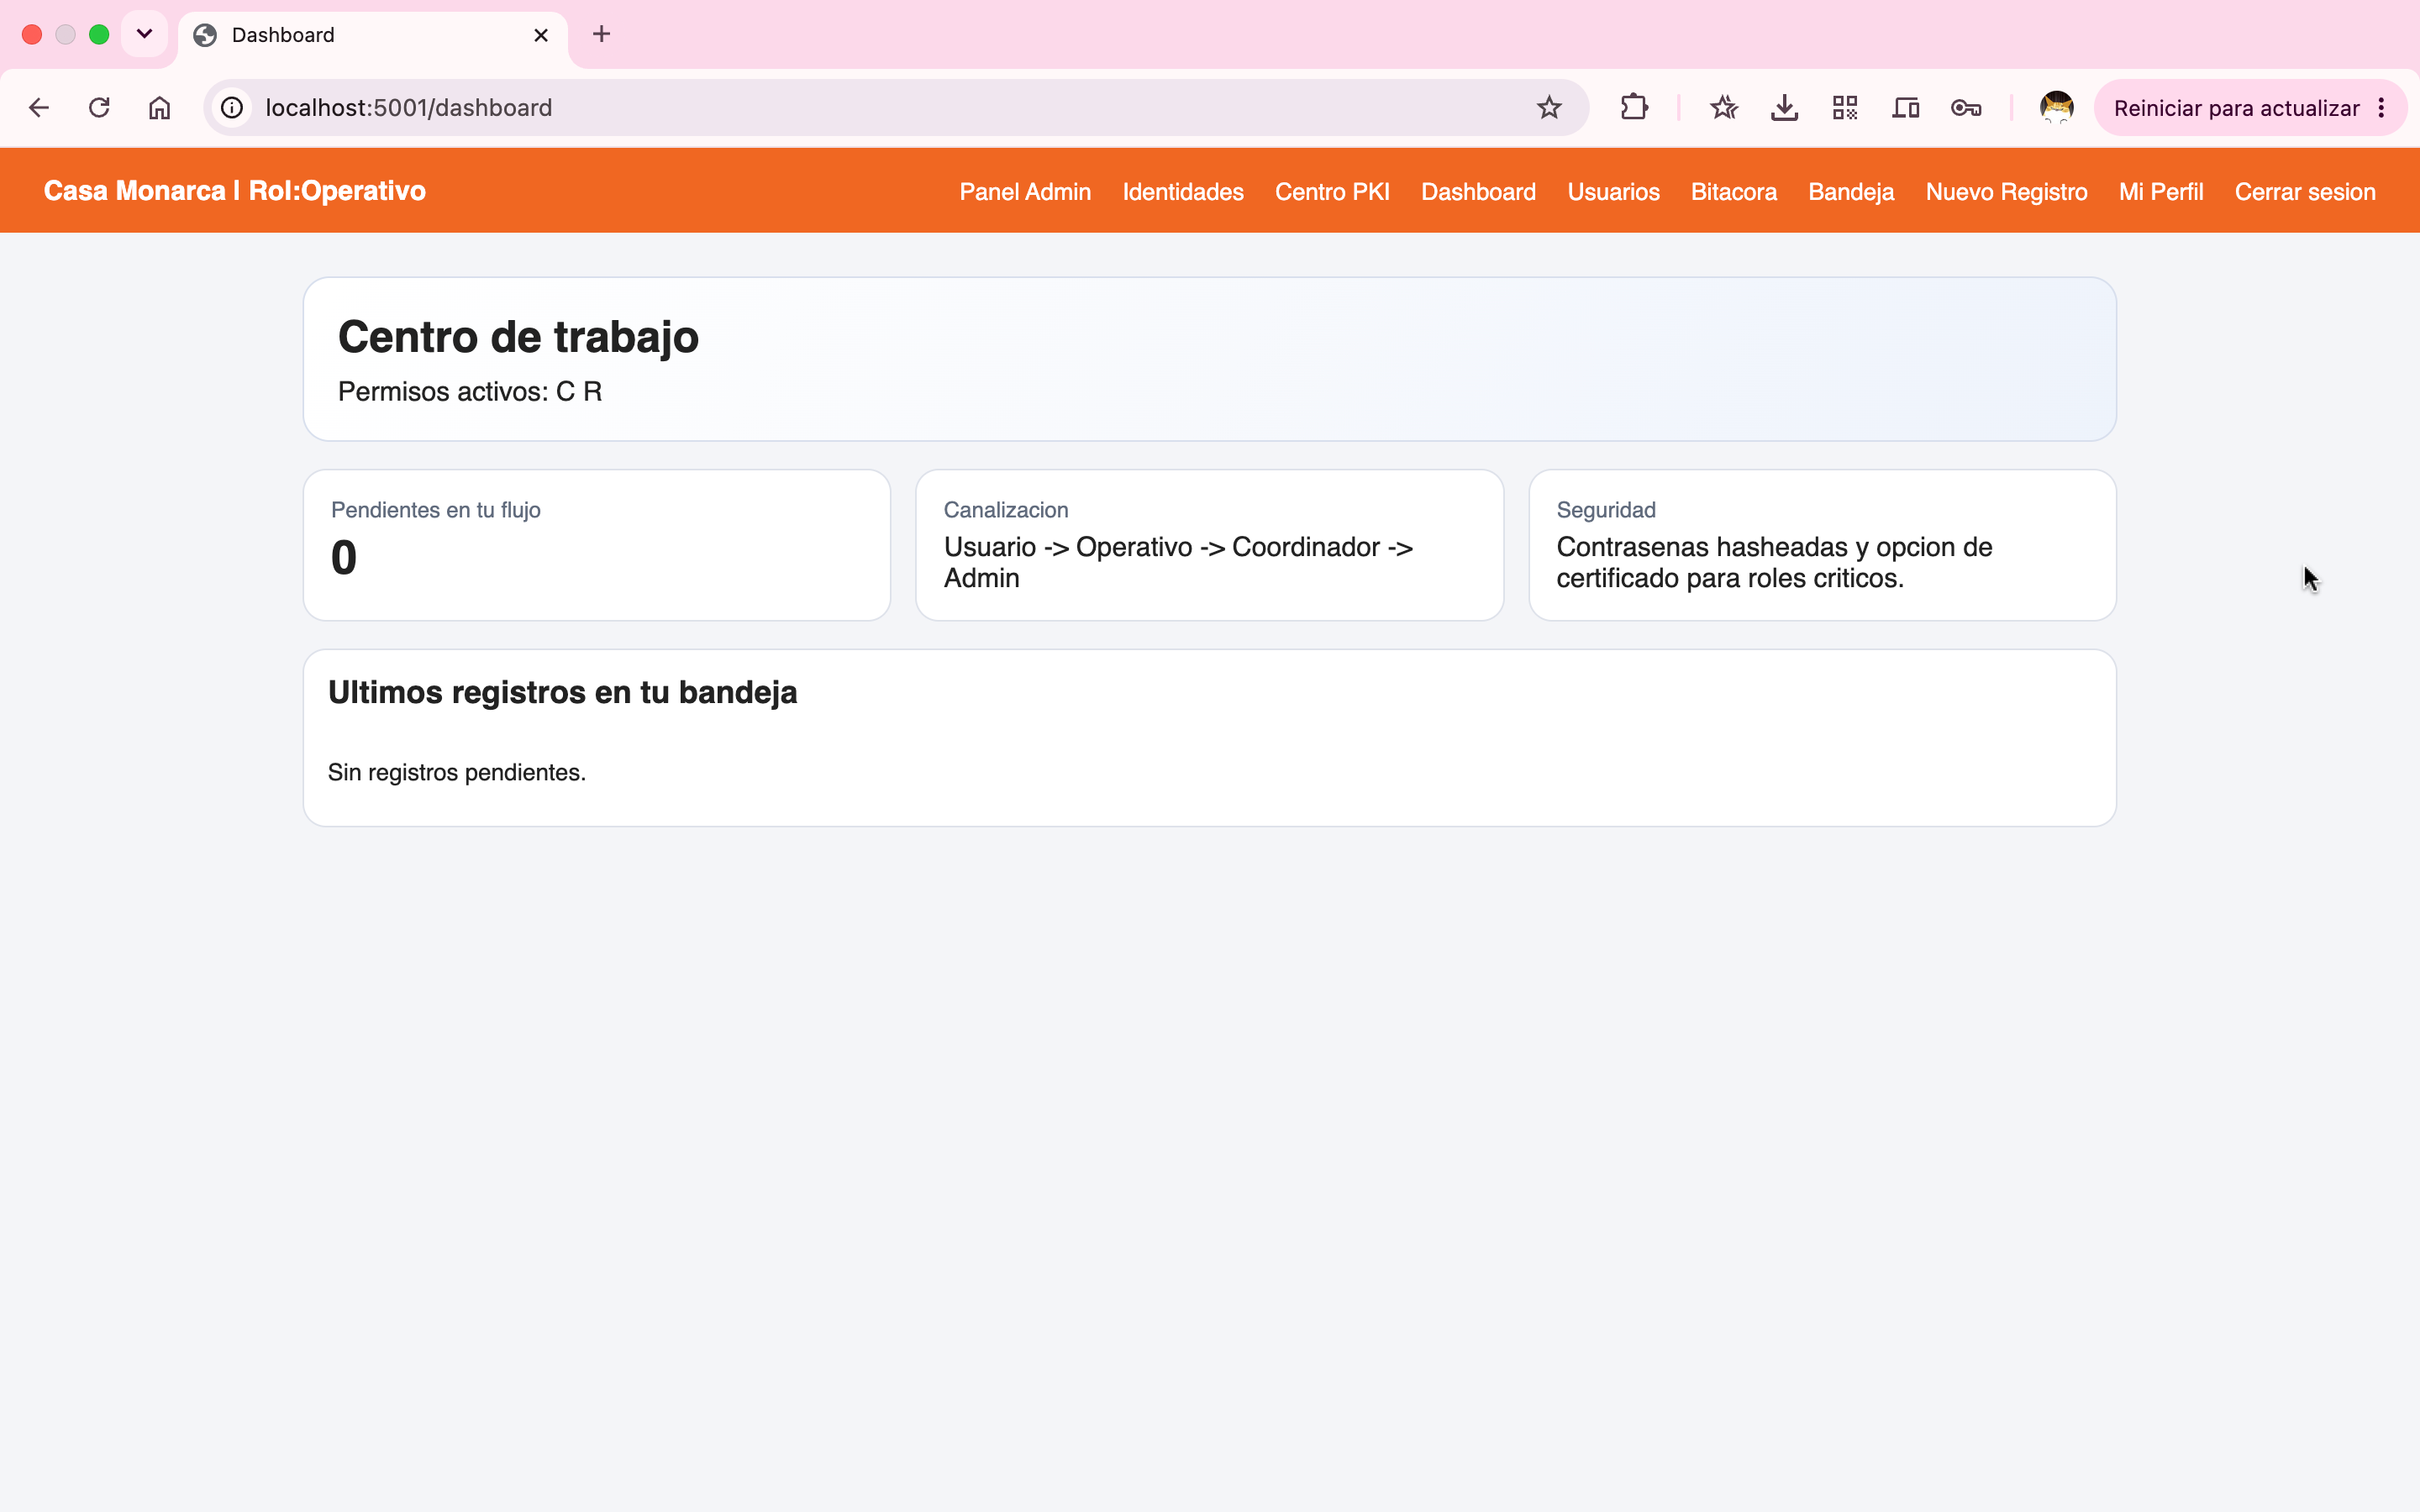
\includegraphics[width=9cm]{Captura de pantalla 2026-06-12 a la(s) 3.47.12 a.m..png}
\\
\midrule

Inicio de sesión con passkey para roles altos
&
Correcto
&
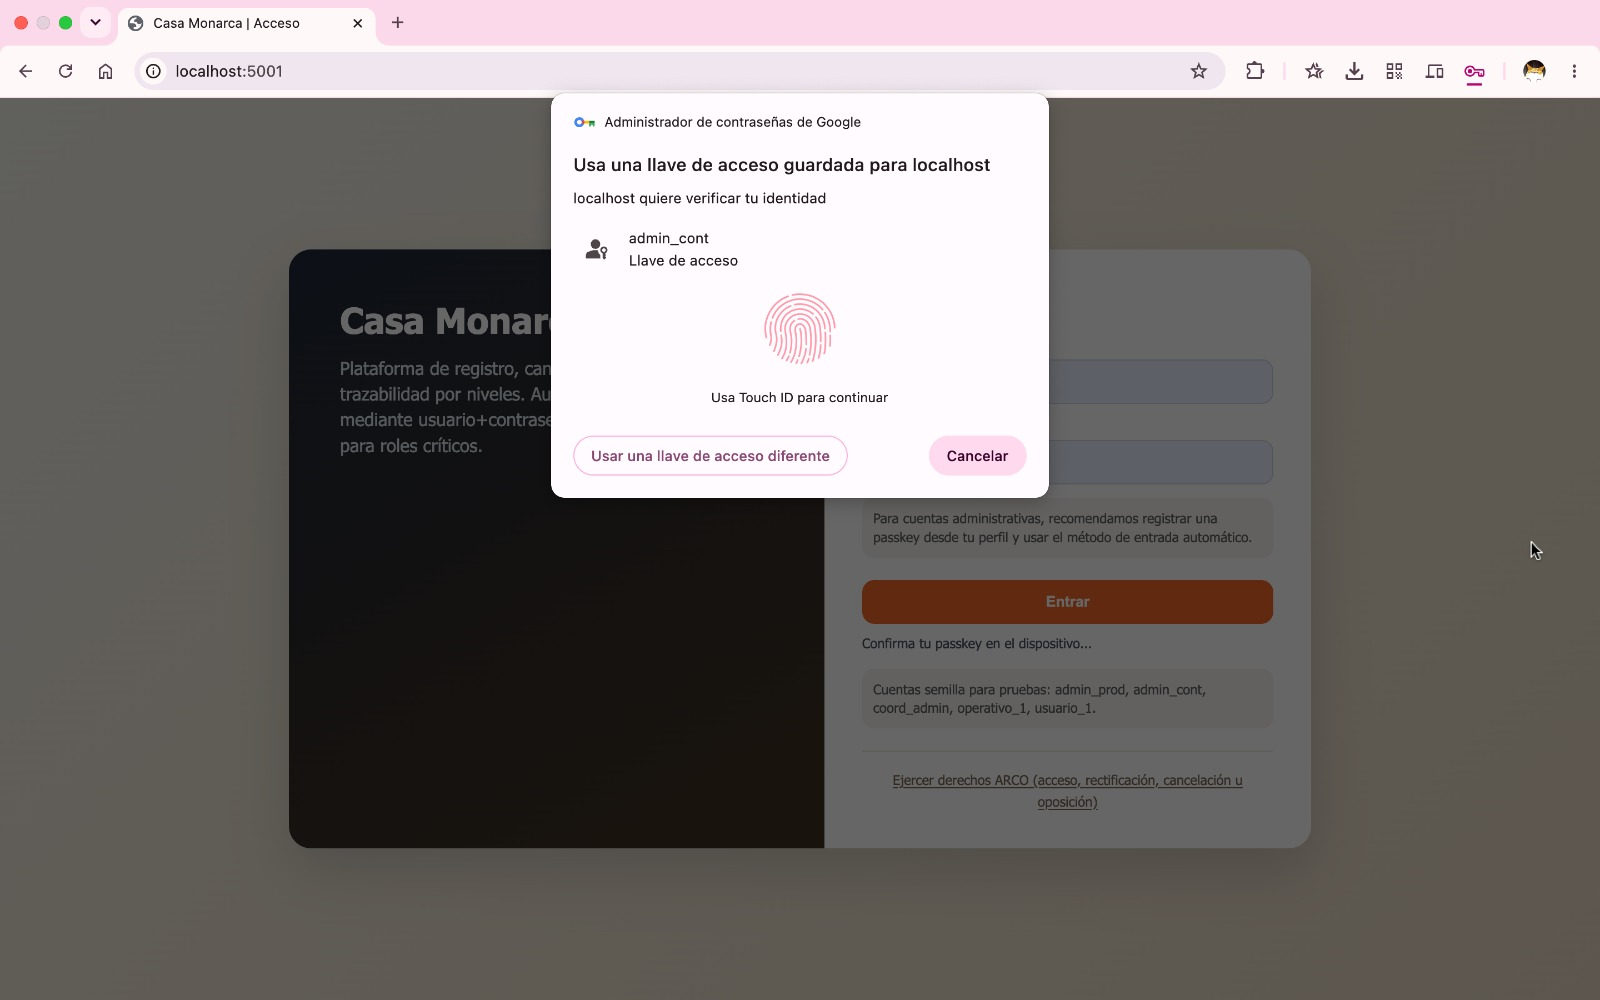
\includegraphics[width=9cm]{WhatsApp Image 2026-06-05 at 7.53.43 PM (4).jpeg}
\\
\midrule

Creación de expediente
&
Correcto
&
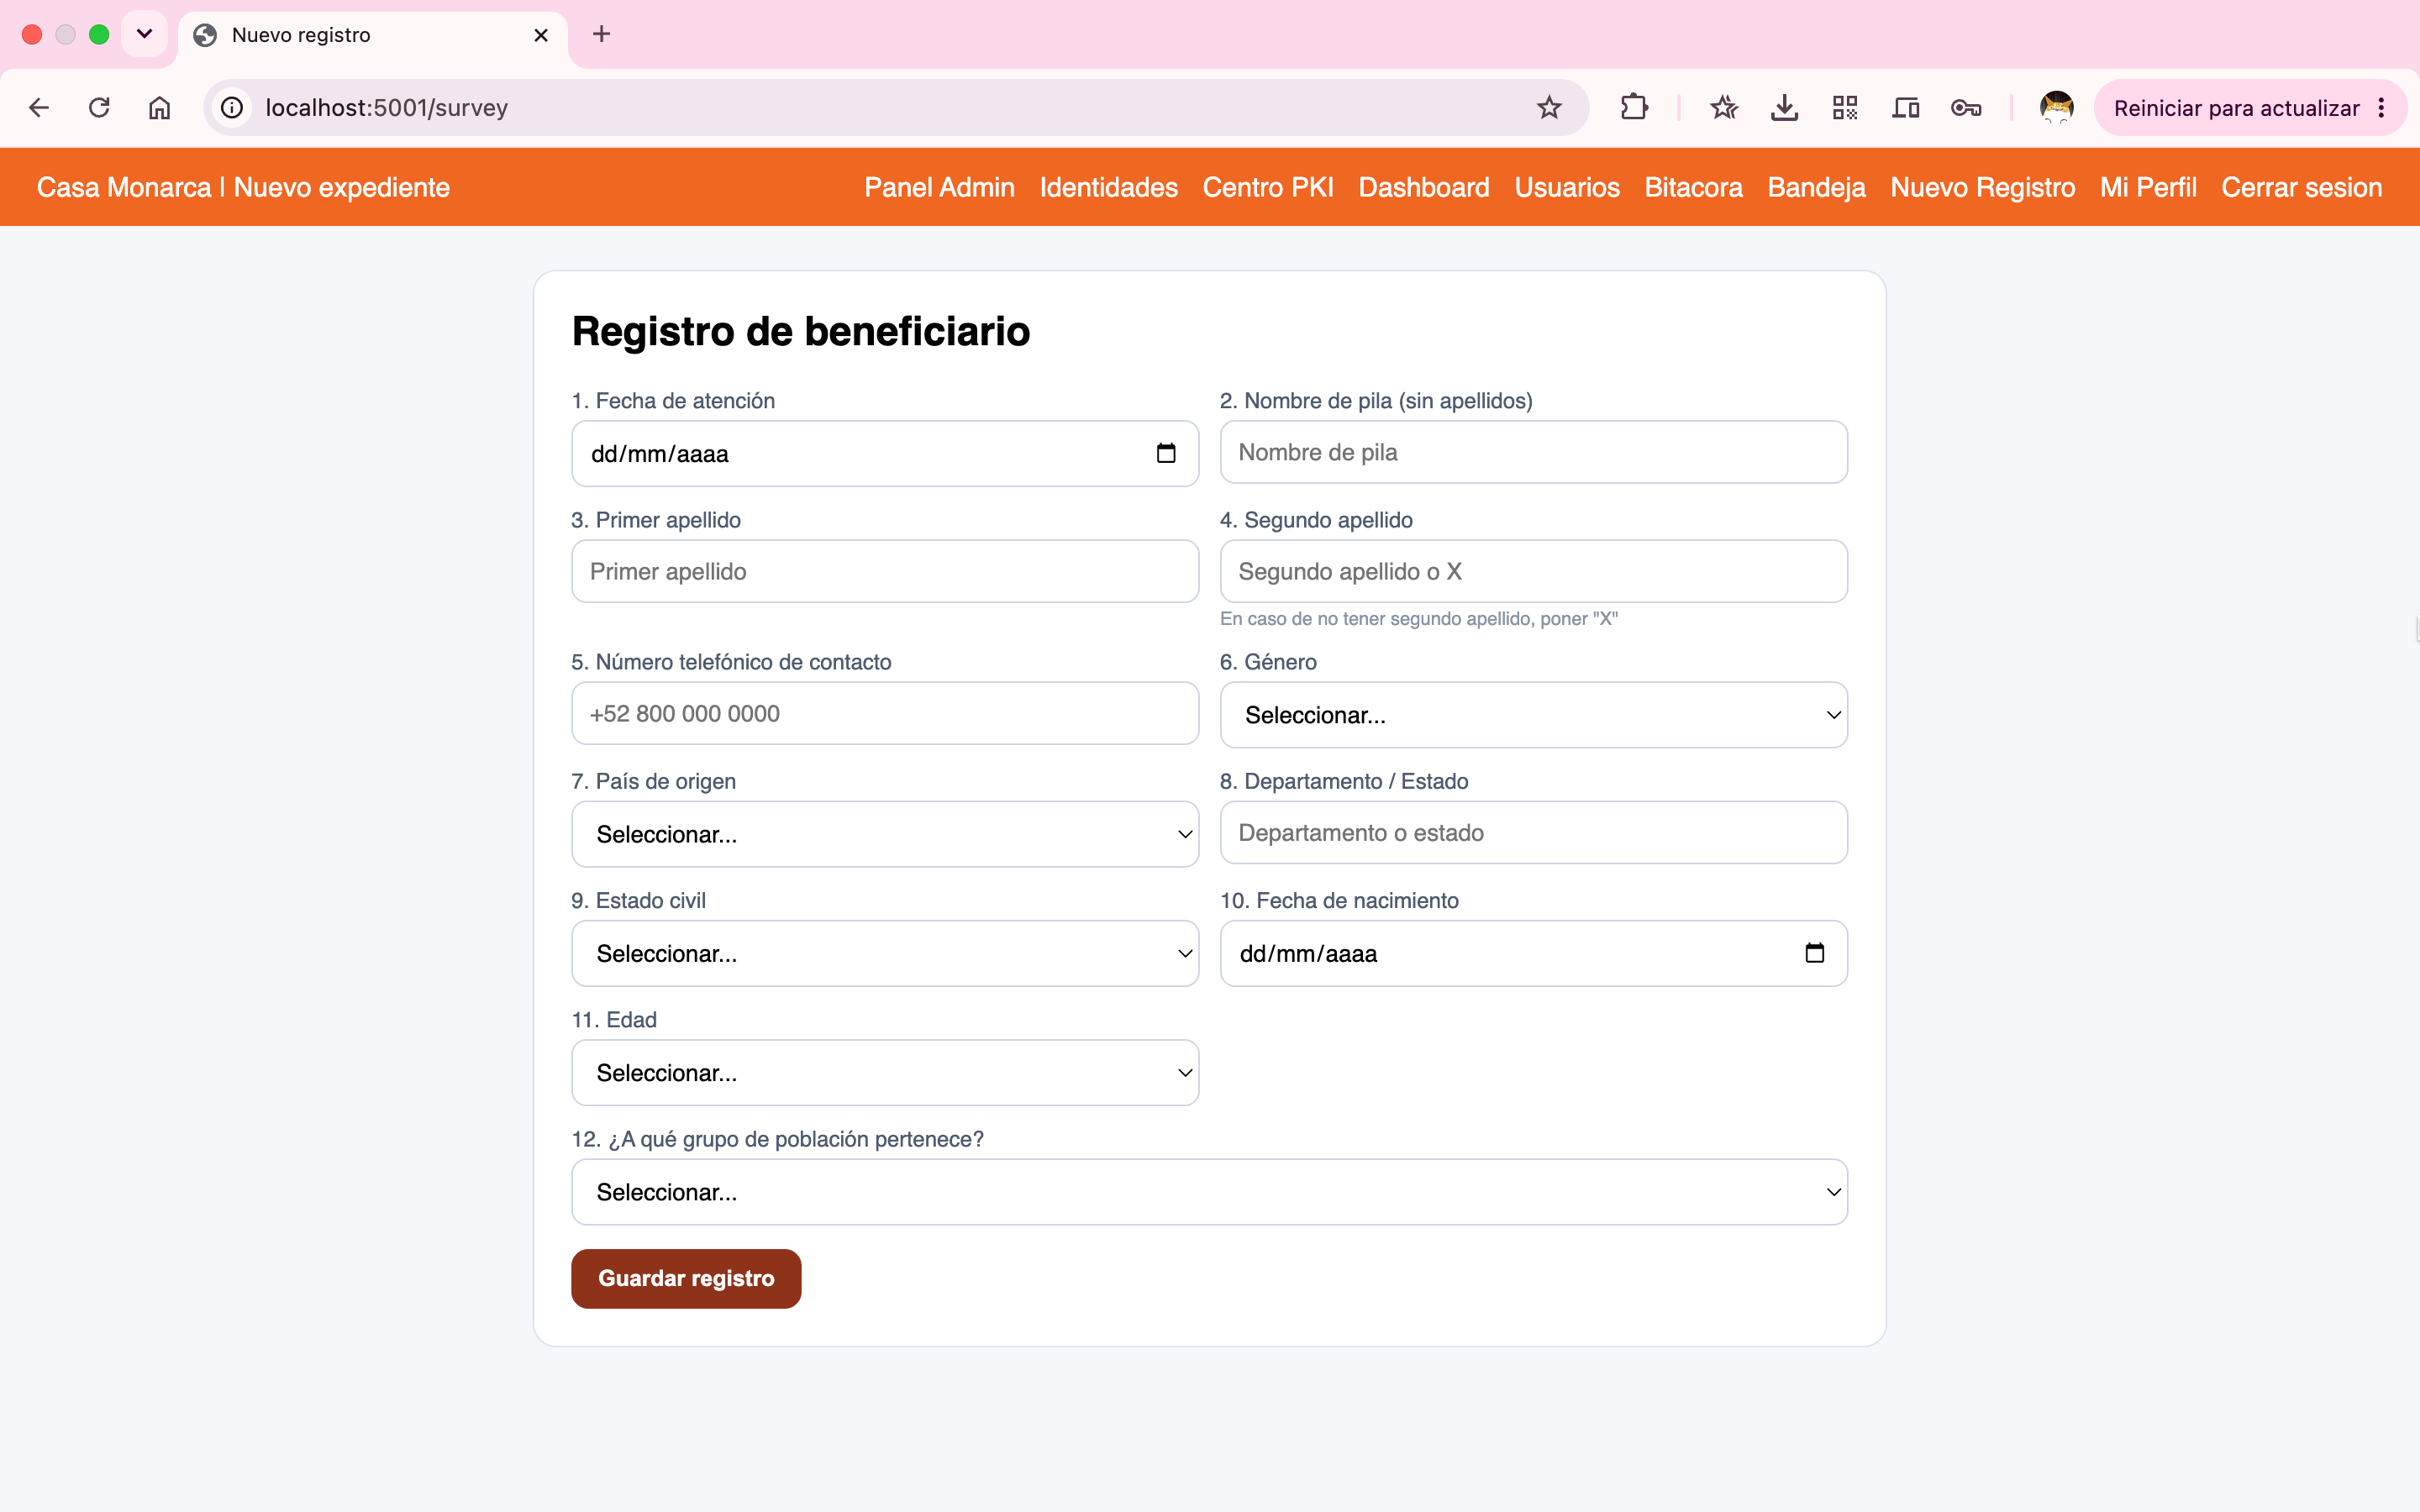
\includegraphics[width=9cm]{Captura de pantalla 2026-06-12 a la(s) 3.48.58 a.m..png}
\\
\midrule

Cifrado de datos en la base de datos
&
Correcto
&
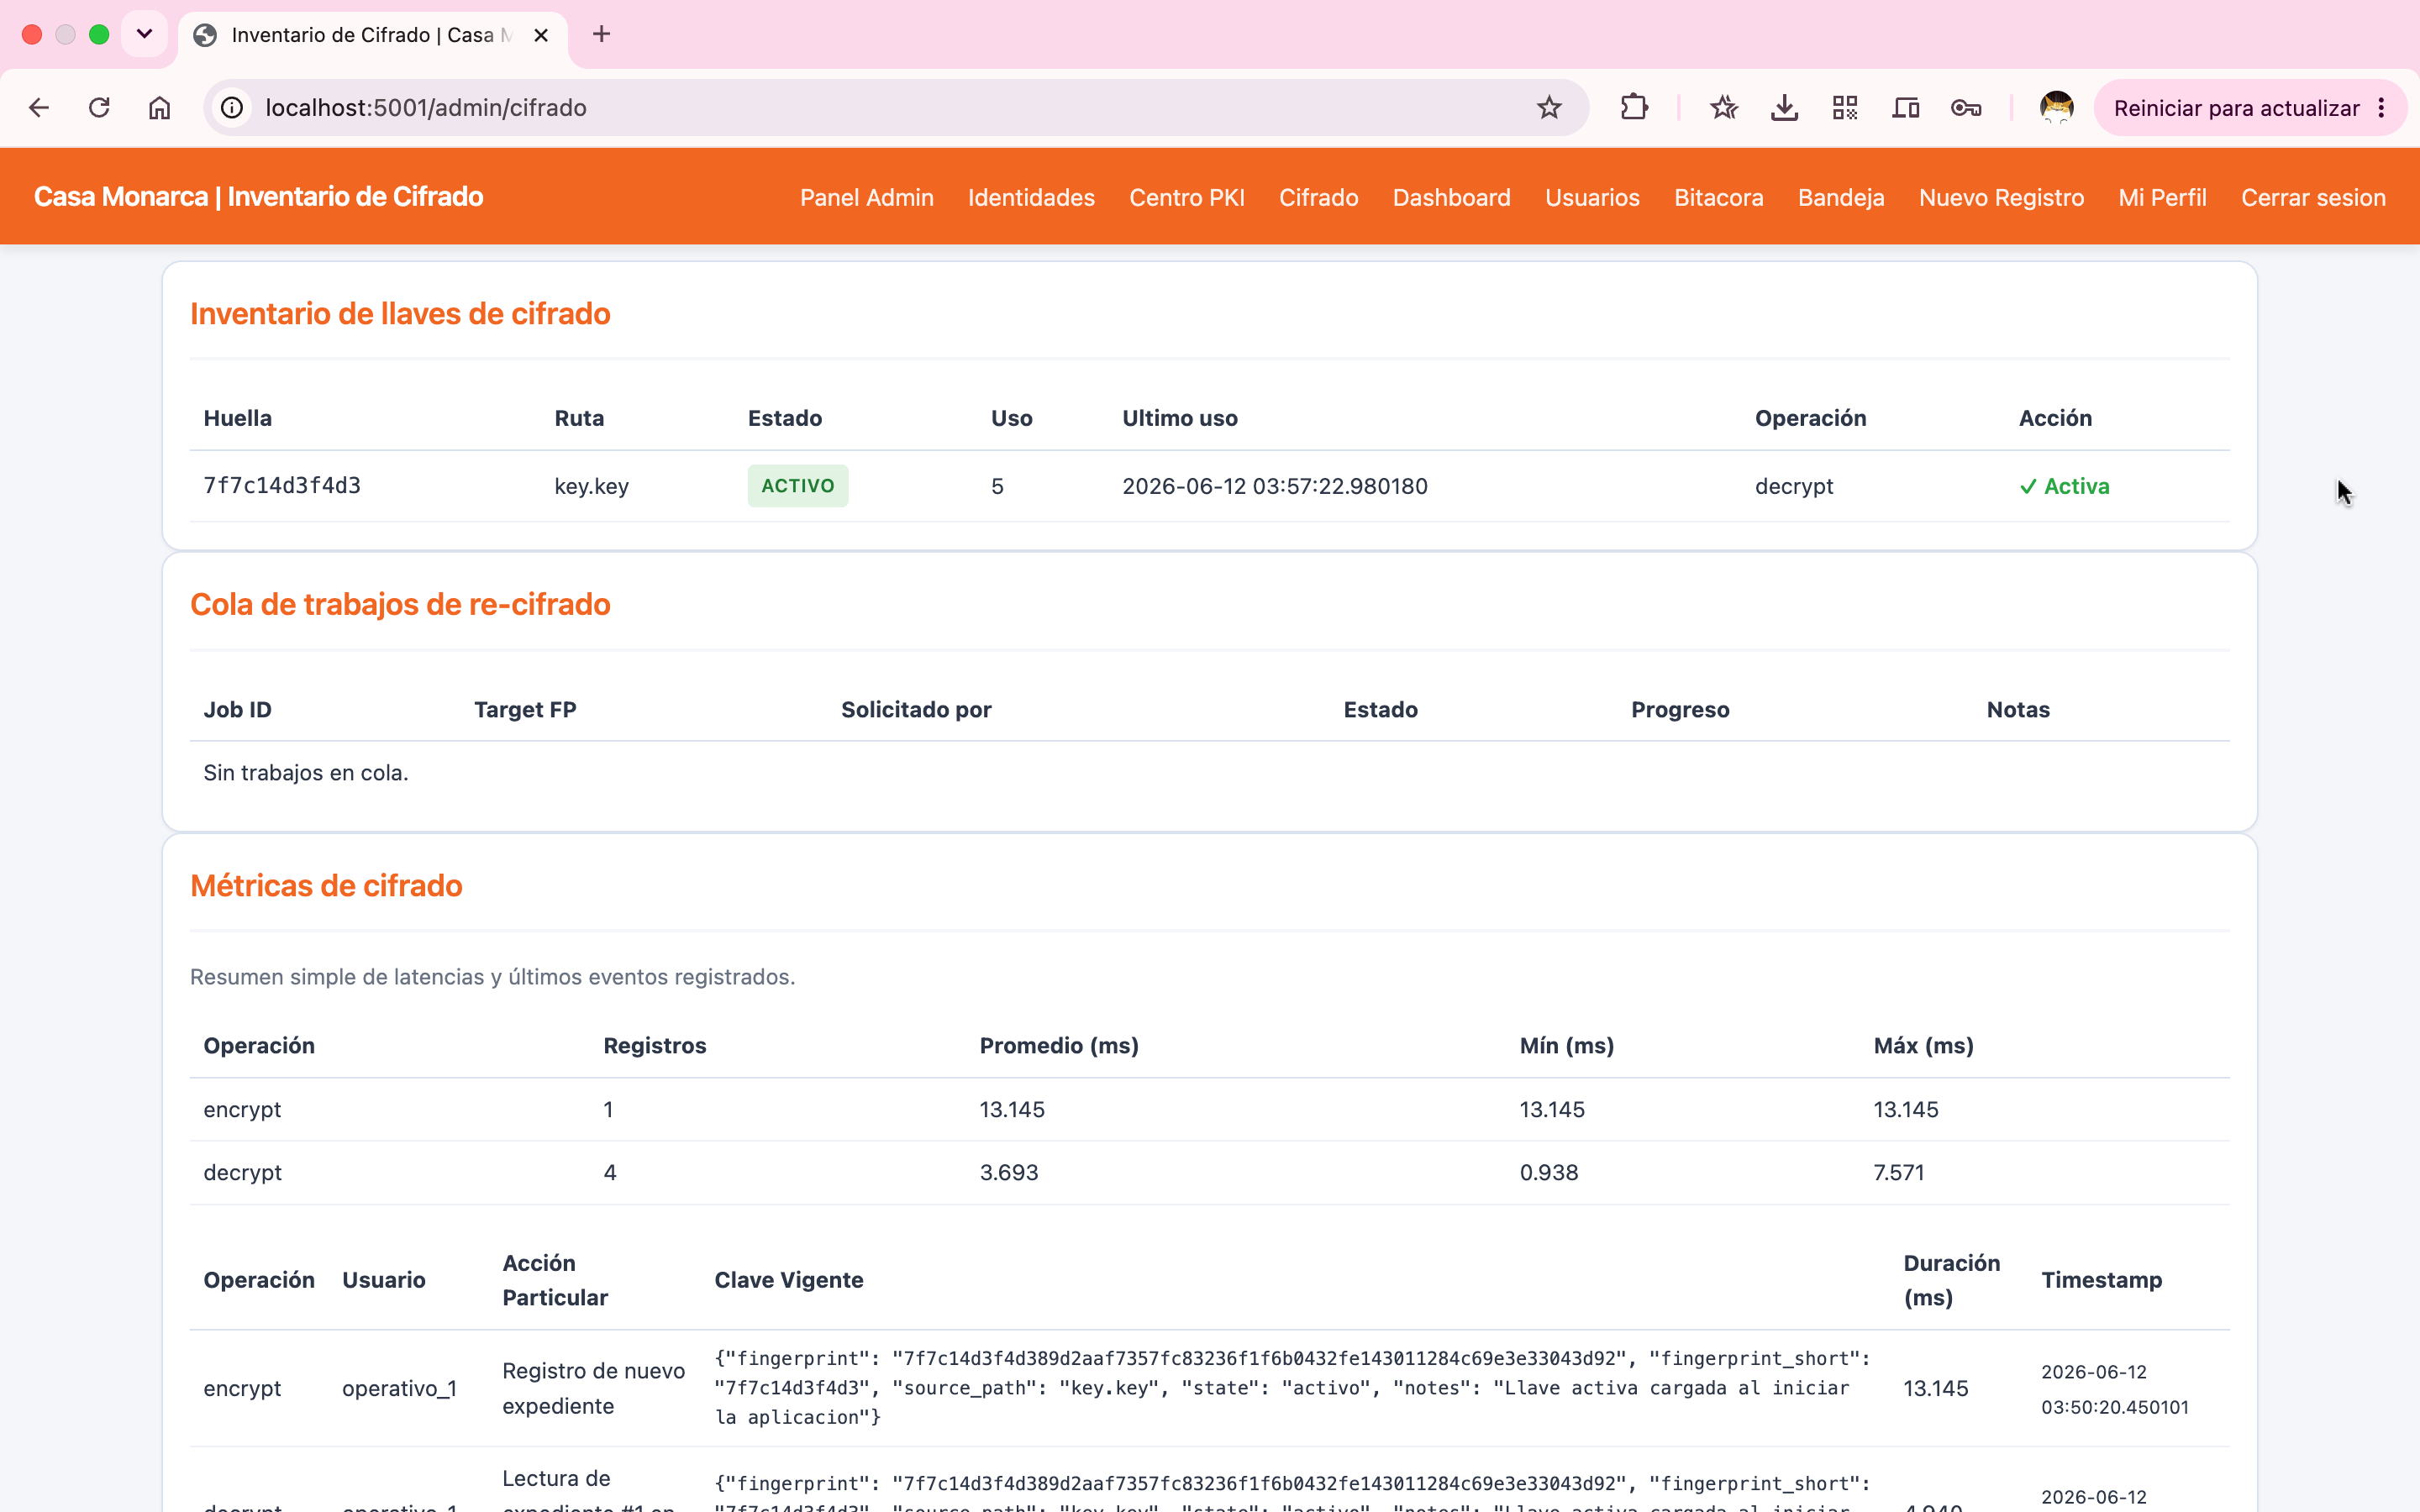
\includegraphics[width=9cm]{Captura de pantalla 2026-06-12 a la(s) 3.57.48 a.m..png}
\\
\midrule

Avance de expediente según rol
&
Correcto
&
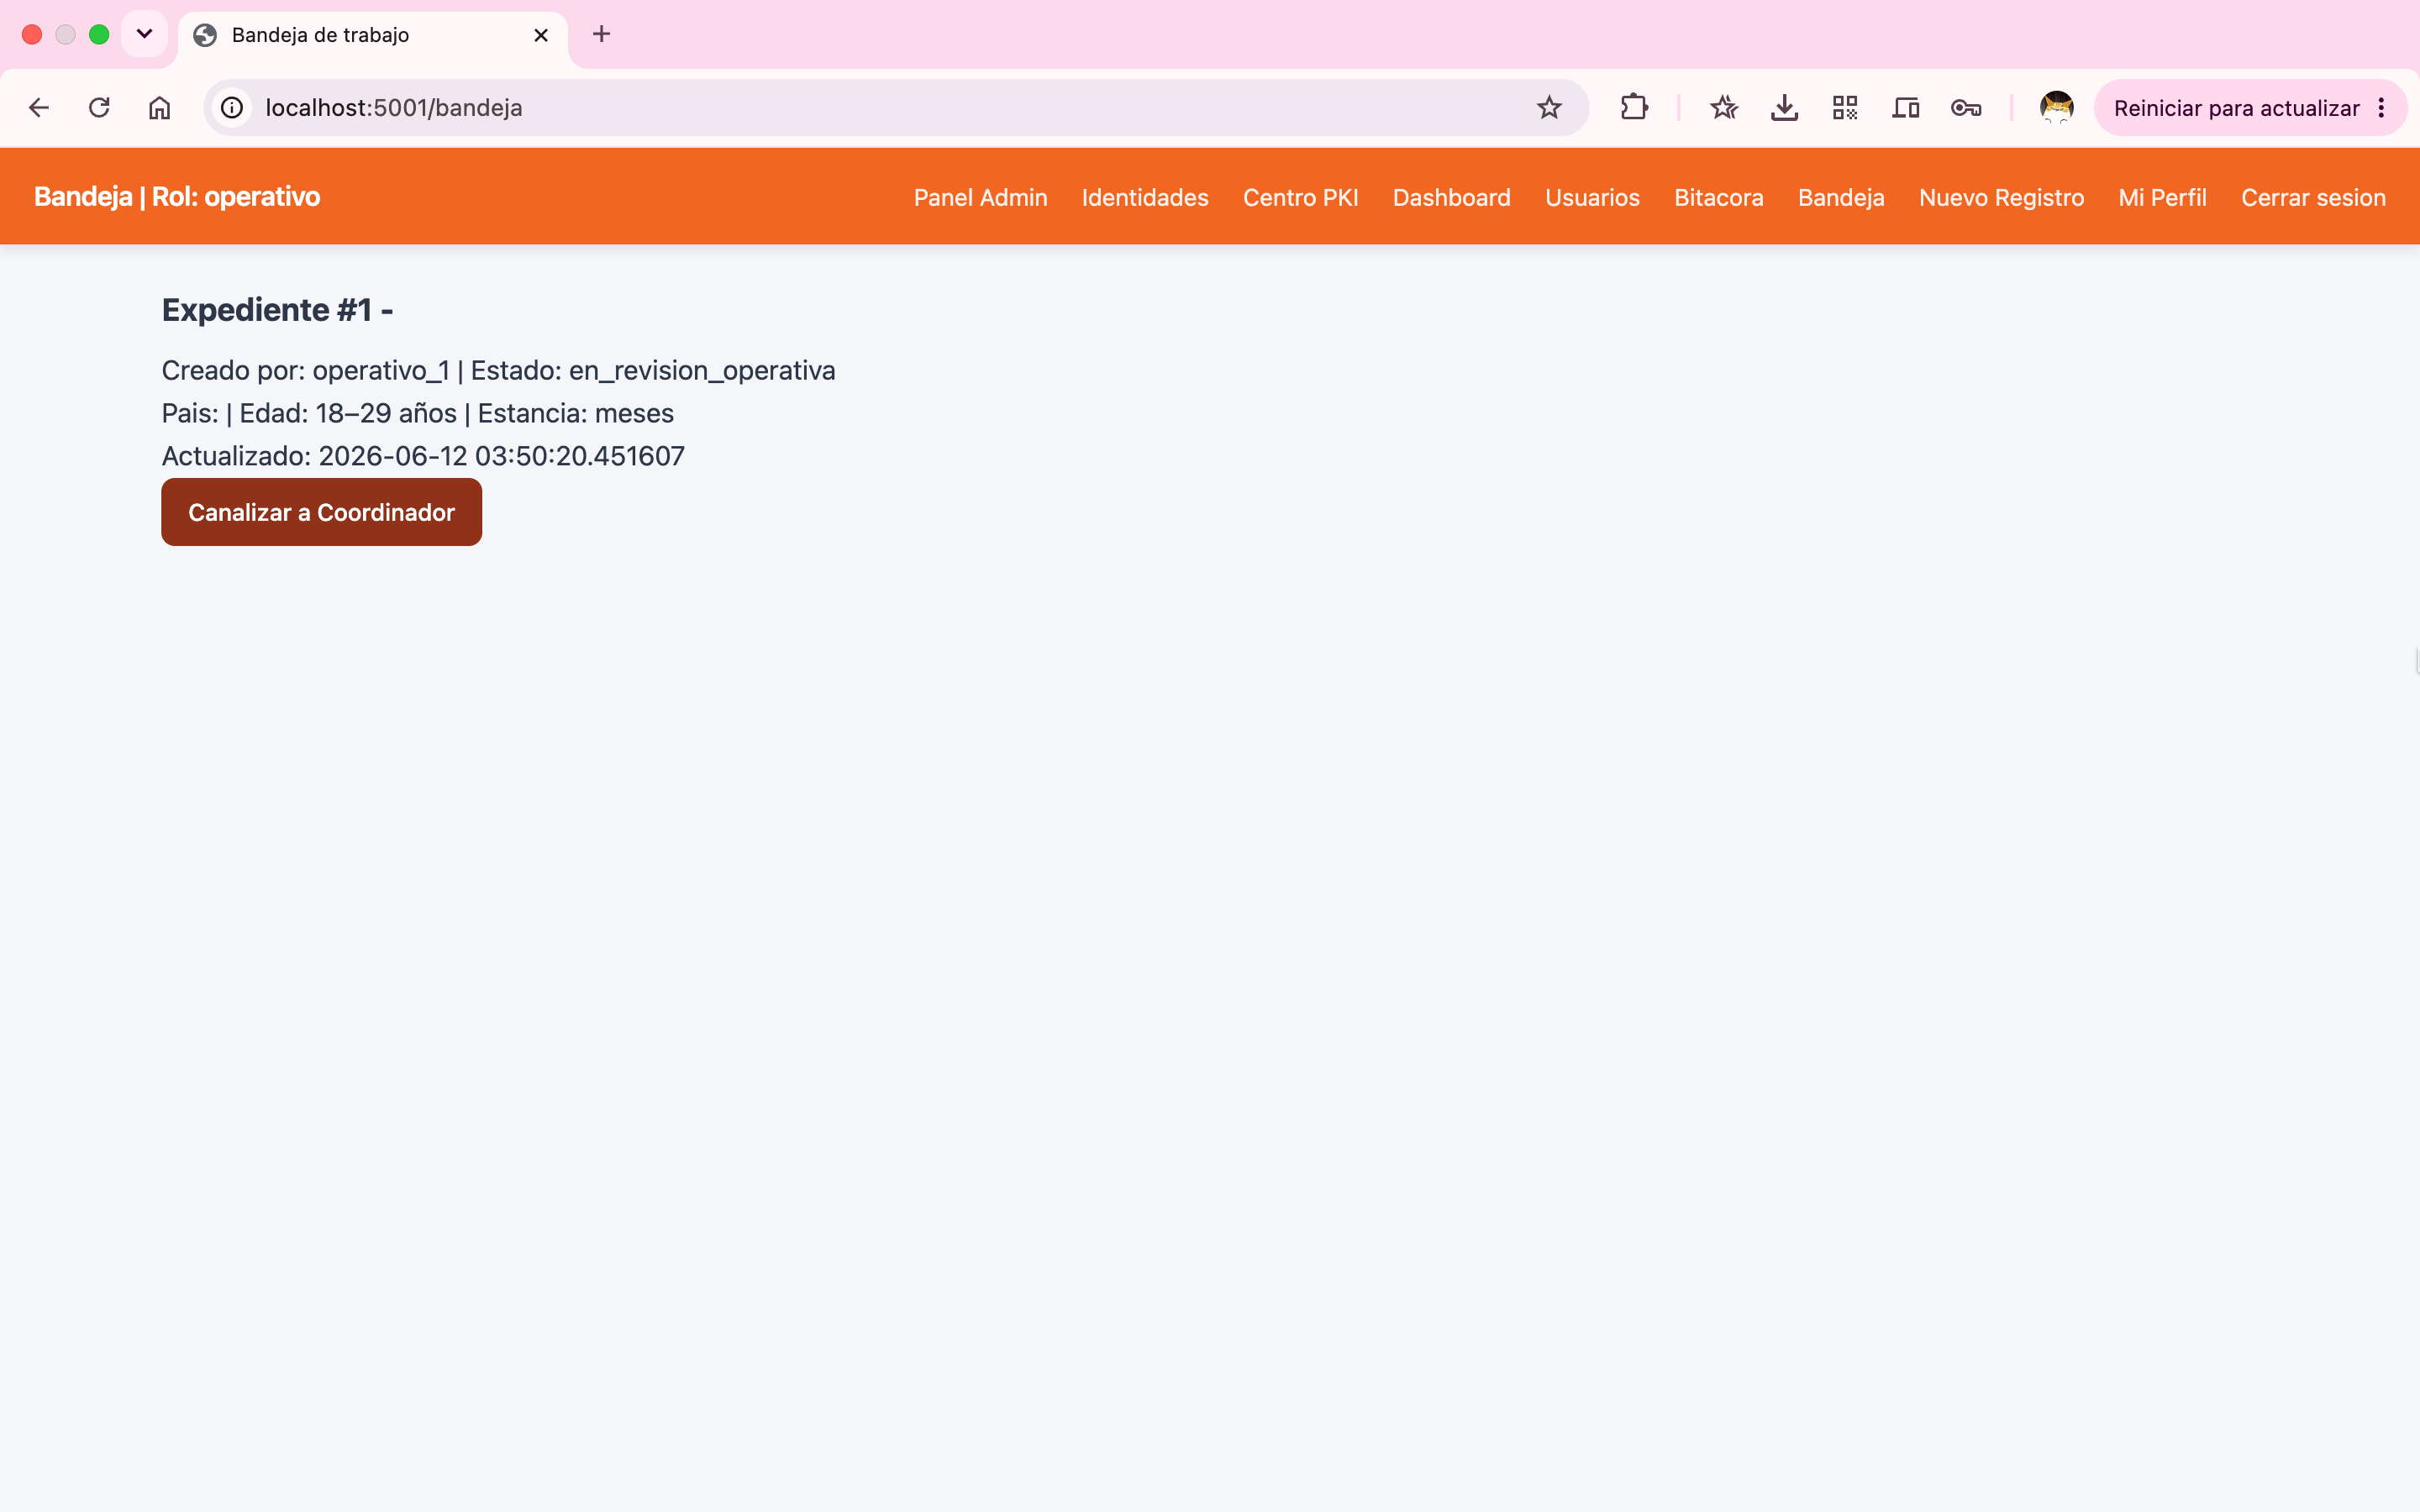
\includegraphics[width=9cm]{Captura de pantalla 2026-06-12 a la(s) 3.50.33 a.m..png}
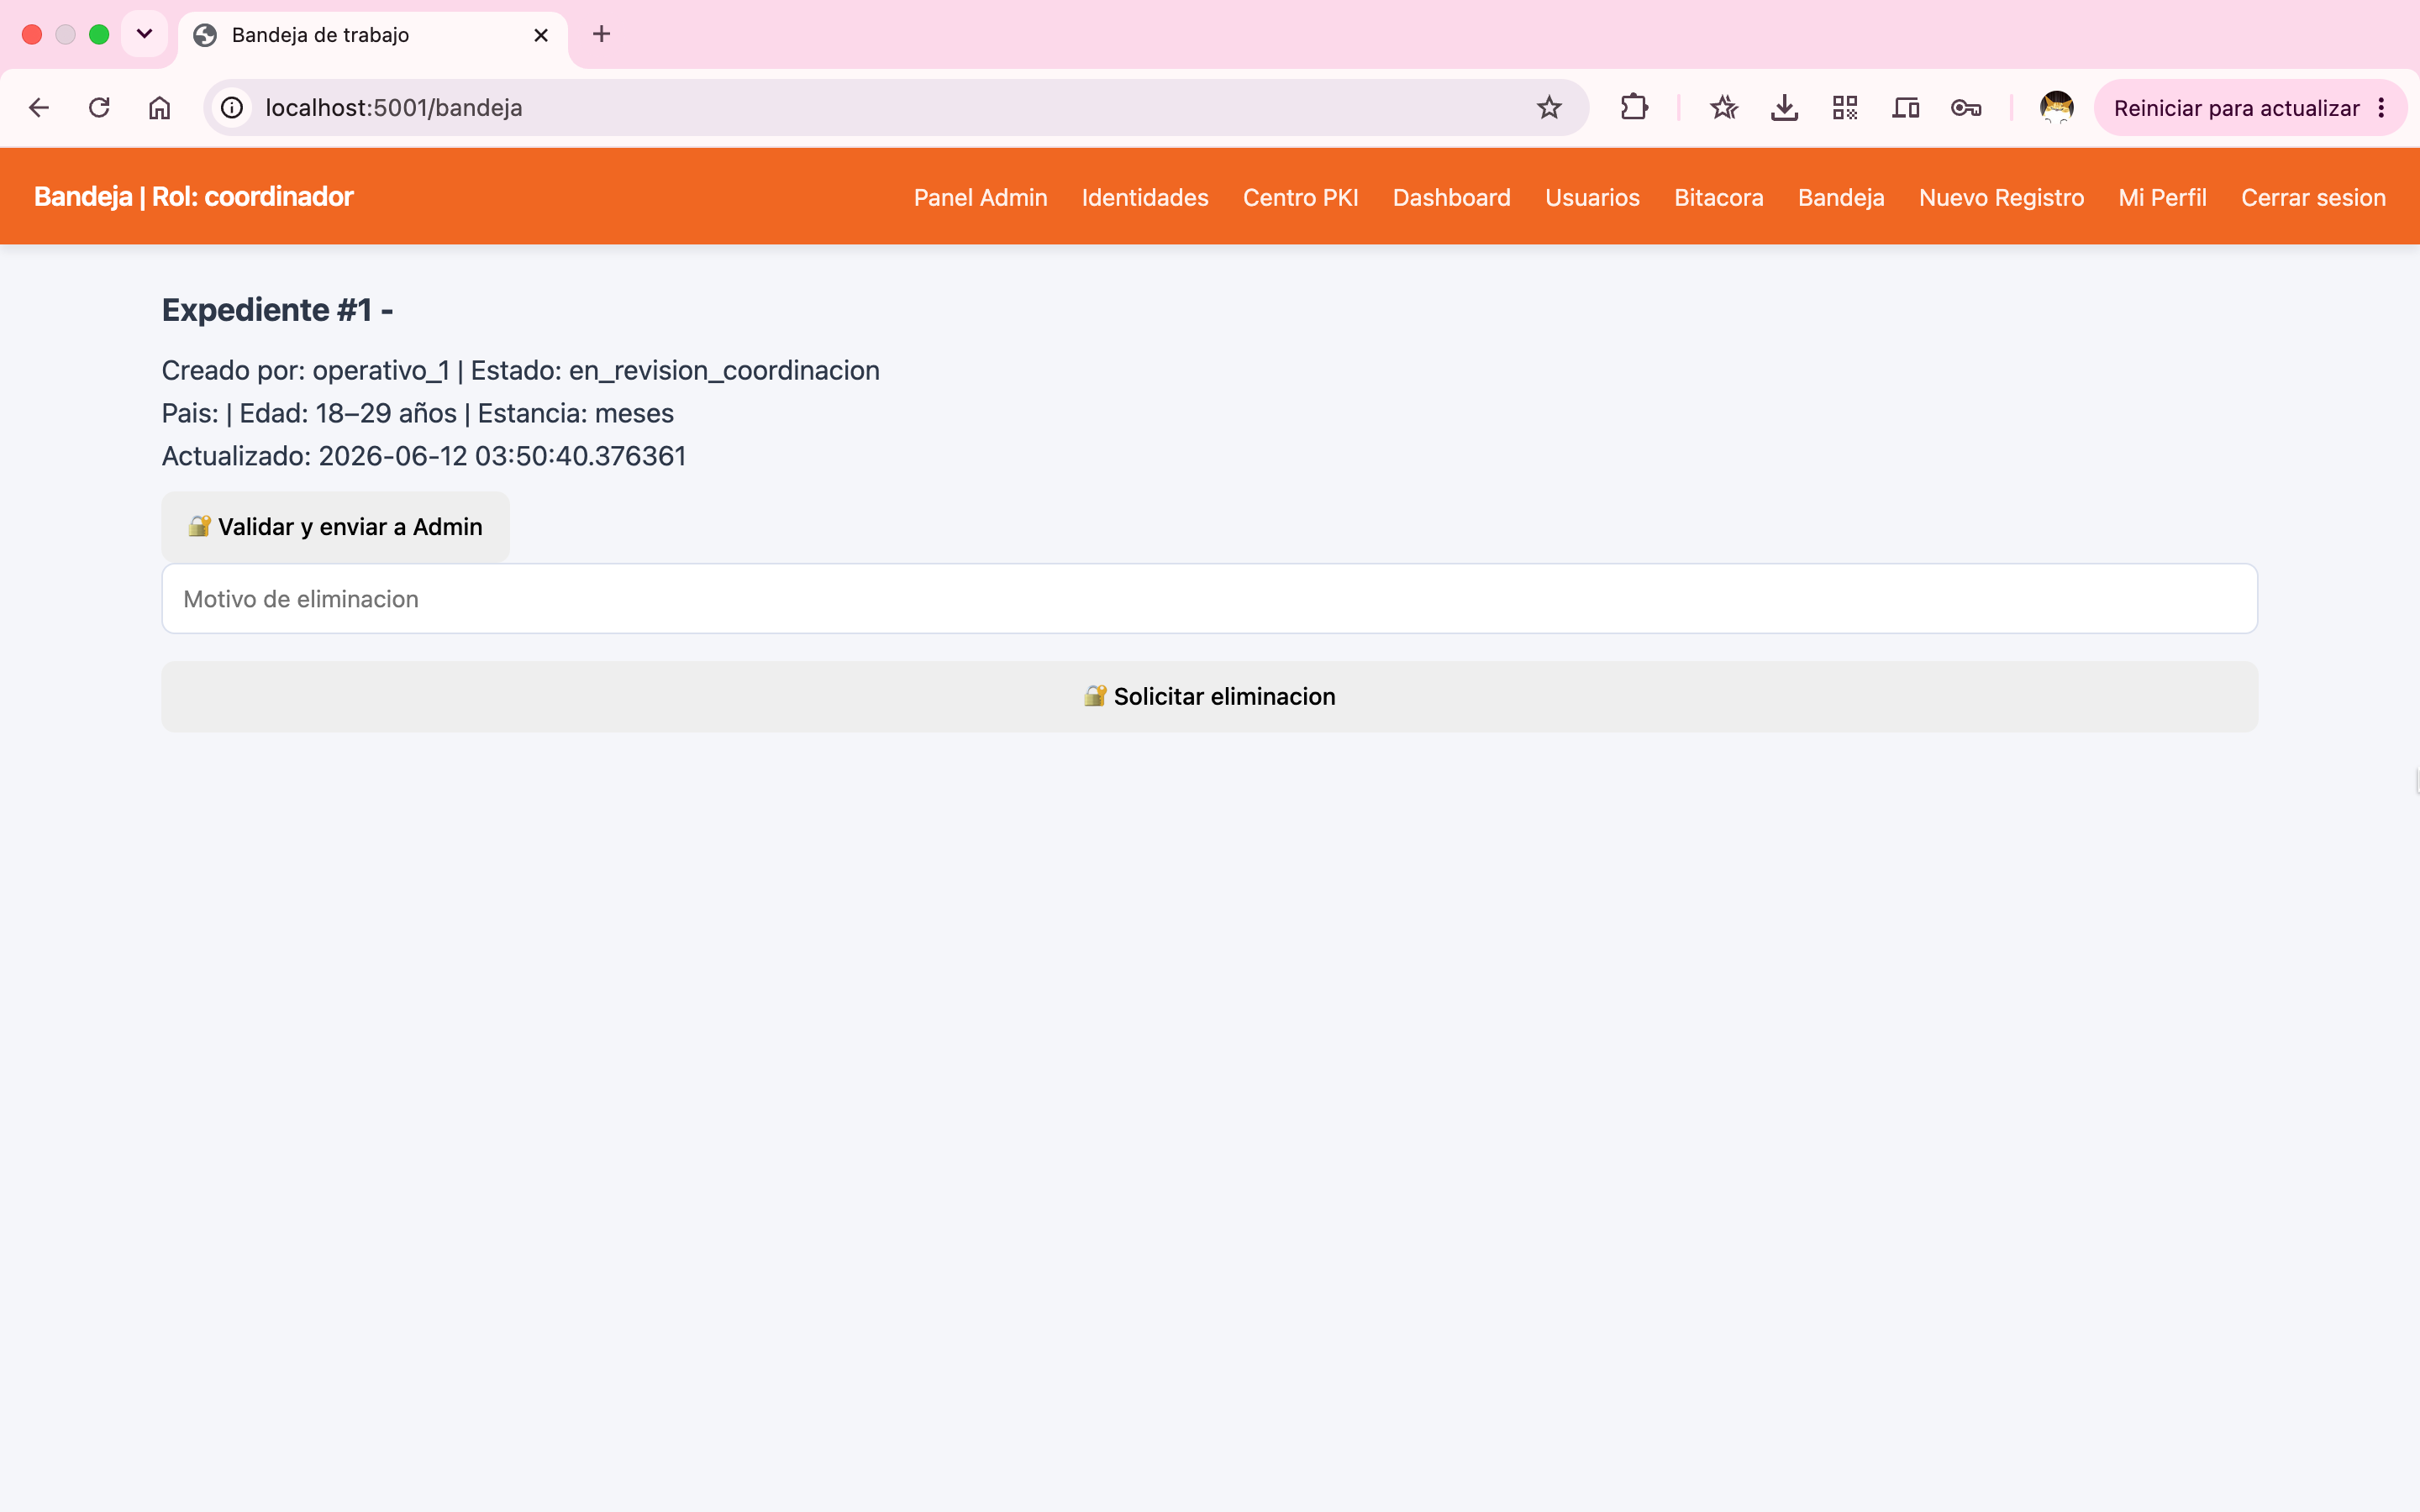
\includegraphics[width=9cm]{Captura de pantalla 2026-06-12 a la(s) 3.51.50 a.m..png}
\\
\midrule

Registro de acciones en bitácora
&
Correcto
&
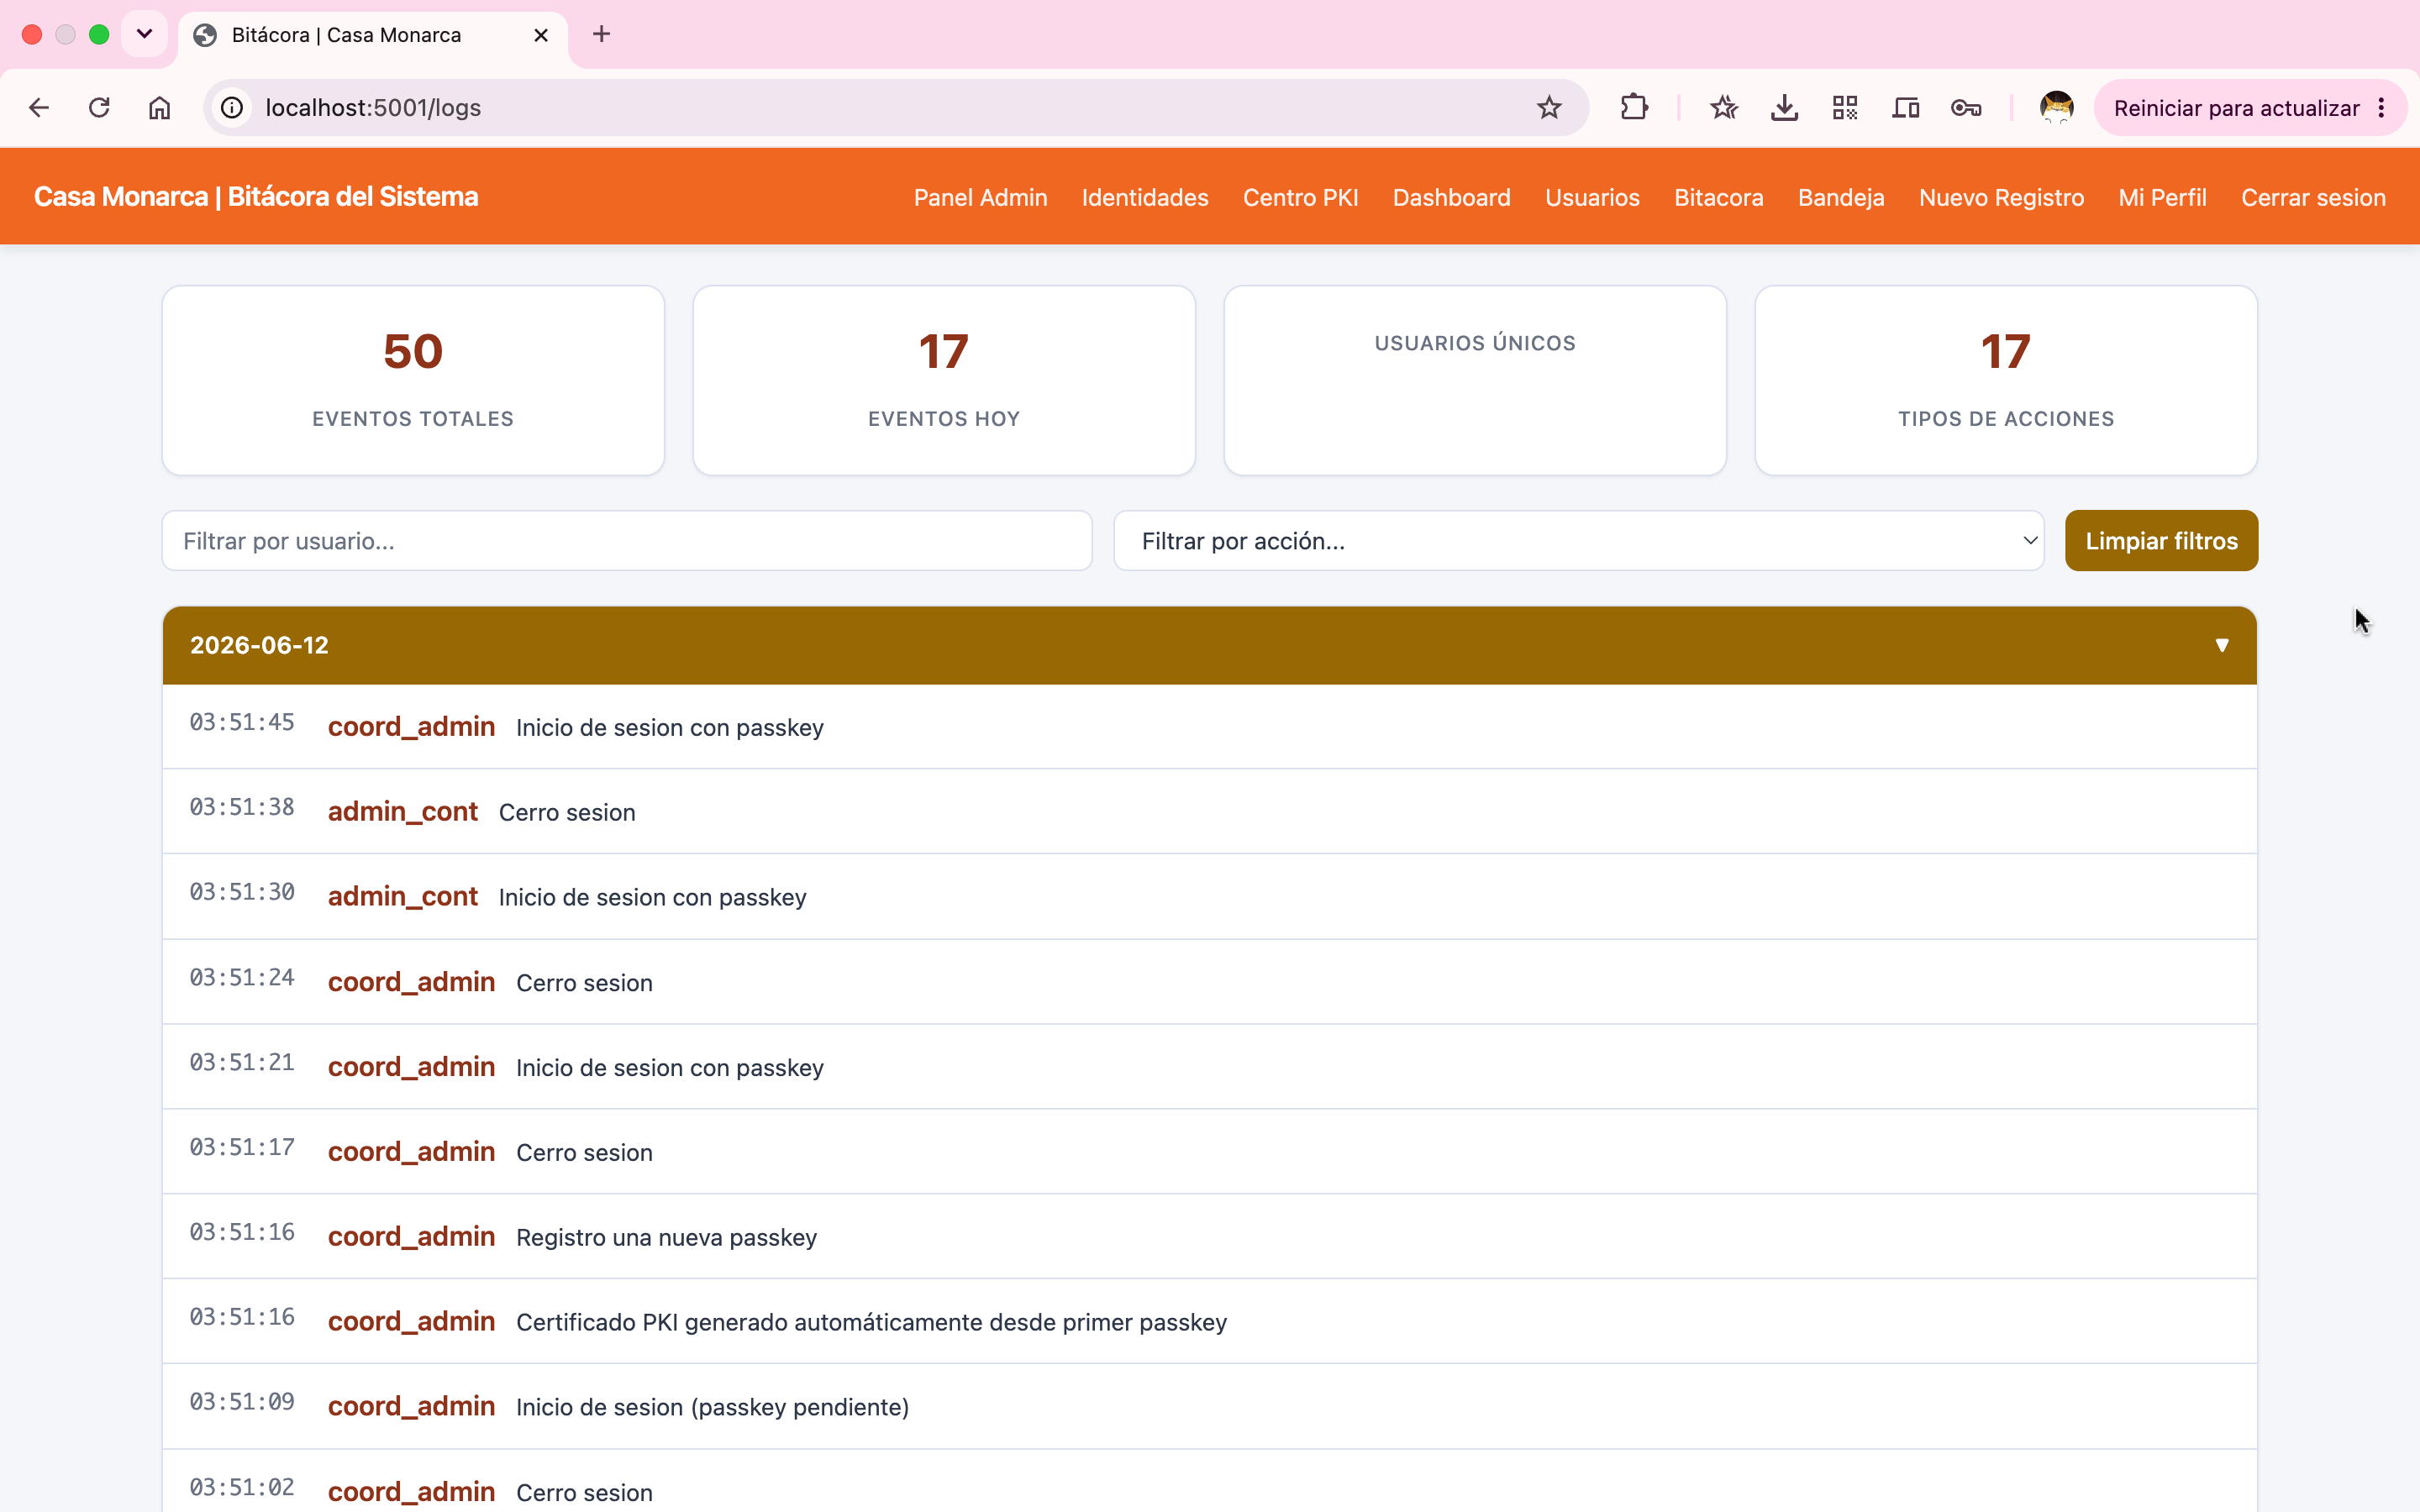
\includegraphics[width=9cm]{Captura de pantalla 2026-06-12 a la(s) 3.54.30 a.m..png}
\\
\midrule

Solicitud ARCO
&
Correcto
&
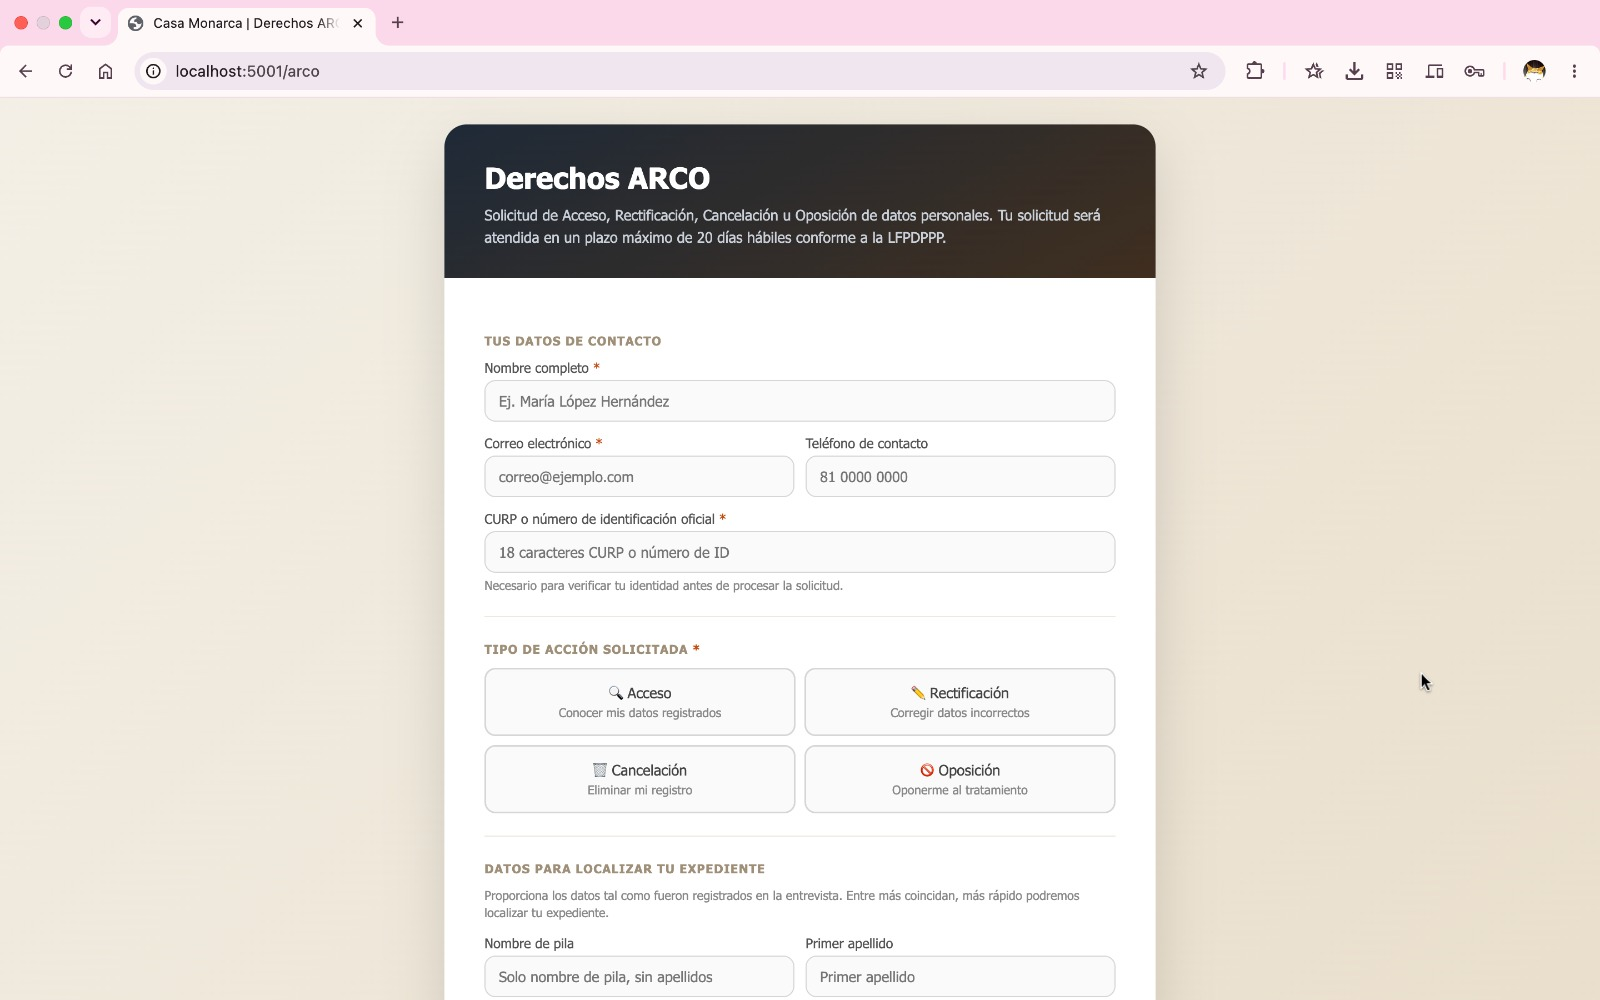
\includegraphics[width=9cm]{WhatsApp Image 2026-06-05 at 7.53.43 PM.jpeg}
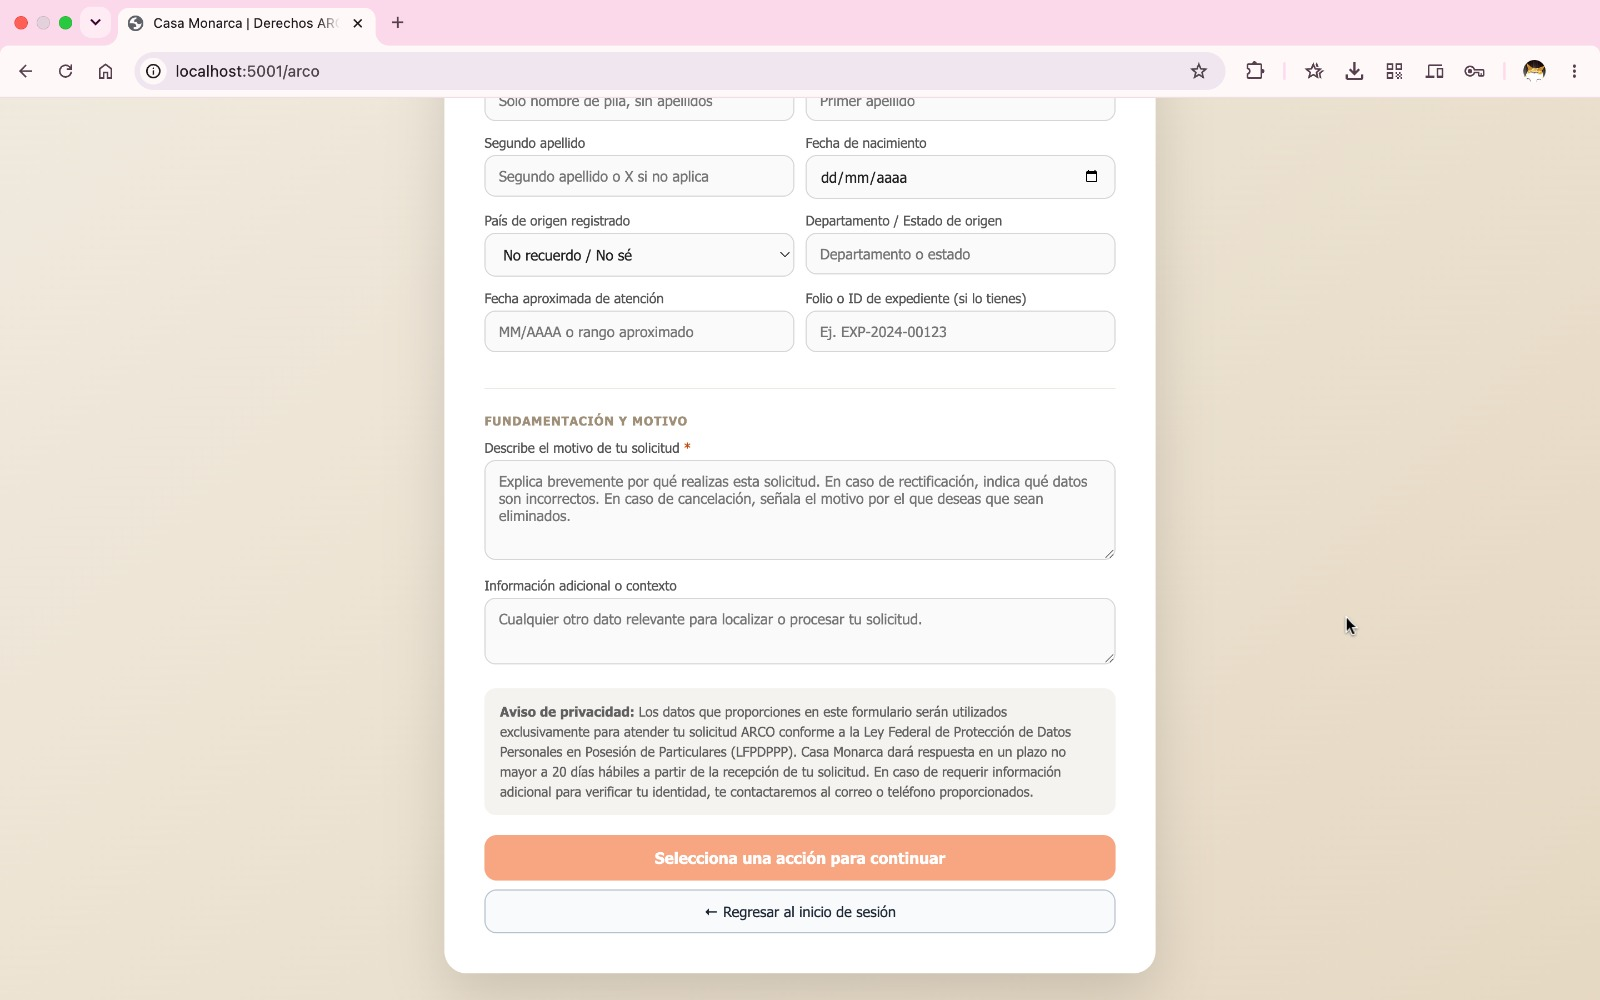
\includegraphics[width=9cm  ]{WhatsApp Image 2026-06-05 at 7.53.43 PM (10).jpeg}
\\

\bottomrule
\caption{Casos de uso y validaciones realizadas.}
\label{tab:validaciones}
\end{longtable}
\end{center}


\newpage

\section{Conclusiones y trabajo futuro}

El desarrollo de este proyecto permitió aplicar conceptos de criptografía, control de acceso y protección de datos personales en una solución orientada a una necesidad real. Mediante la integración de certificados digitales X.509, autenticación reforzada con passkeys (WebAuthn), cifrado de información sensible mediante Fernet y un sistema de auditoría, fue posible construir una plataforma que fortalece la seguridad en la gestión de expedientes digitales. La arquitectura implementada permite proteger la confidencialidad de la información, controlar los accesos y mantener un registro de las acciones realizadas dentro del sistema.

Además de mejorar la organización y administración de los expedientes, la solución contribuye a fortalecer la cultura de protección de datos dentro de la organización. La incorporación de solicitudes ARCO y el registro automático de eventos permiten contar con mecanismos de transparencia, trazabilidad y rendición de cuentas alineados con la Ley General de Protección de Datos Personales. Esto reduce riesgos asociados al acceso no autorizado o a la manipulación indebida de información sensible, ya que cada acción queda vinculada a un usuario y a un conjunto específico de permisos definidos mediante el modelo RBAC.

La ejecución de este proyecto también representó una experiencia distinta a otros desarrollos realizados durante la carrera. A diferencia de proyectos enfocados en inventarios, rutas o análisis de datos, en este caso se trabajó con información personal sensible, lo que implicó asumir una responsabilidad adicional durante el diseño e implementación de la solución. Esto permitió comprender la importancia de incorporar la seguridad desde las primeras etapas del desarrollo y no únicamente como una característica adicional al final del proyecto.

Asimismo, este trabajo fue el resultado de un proceso de análisis, diseño, implementación y validación que se desarrolló a lo largo de un semestre. Durante este periodo se abordaron distintos retos técnicos, como la gestión de llaves criptográficas, la implementación de passkeys mediante WebAuthn, la integración de certificados digitales y el diseño de mecanismos de auditoría y control de acceso. Estos desafíos permitieron trasladar conceptos teóricos de seguridad a una implementación funcional orientada a resolver una problemática real.

De igual forma, el proyecto demostró que es posible integrar mecanismos avanzados de seguridad sin afectar significativamente la experiencia de uso de los distintos perfiles de usuario. Esto resulta especialmente importante en organizaciones como Casa Monarca, donde las herramientas tecnológicas deben ser accesibles para personas con distintos niveles de experiencia técnica. En este sentido, la solución desarrollada sigue principios de privacidad desde el diseño (Privacy by Design), incorporando medidas de protección directamente en la arquitectura del sistema.

Finalmente, el sistema desarrollado proporciona una base tecnológica sobre la cual la organización puede continuar fortaleciendo sus procesos de gestión y protección de información. Más allá de los beneficios operativos, el proyecto demuestra cómo la ingeniería de software puede contribuir a la protección de datos personales y al fortalecimiento de organizaciones que trabajan con poblaciones en situación de vulnerabilidad.

Como trabajo futuro se propone migrar la base de datos hacia un sistema gestor más robusto que permita soportar una mayor cantidad de usuarios y operaciones simultáneas. También se recomienda implementar despliegues bajo HTTPS, automatizar la administración y rotación de llaves criptográficas mediante gestores de secretos, y sustituir las credenciales de prueba por variables de entorno o mecanismos especializados para la gestión segura de credenciales. Adicionalmente, podría incorporarse procesamiento asíncrono para tareas de alto costo computacional, como el recifrado masivo de expedientes, con el fin de mejorar el rendimiento y la disponibilidad del sistema en entornos de producción.


\newpage

\section{Referencias}

\begin{enumerate}

\item Stallings, W. (2023). \textit{Cryptography and Network Security: Principles and Practice} (9th ed.). Pearson.

\item Whitman, M. E., \& Mattord, H. J. (2021). \textit{Principles of Information Security} (7th ed.). Cengage Learning.

\item National Institute of Standards and Technology. (2020). \textit{Security and Privacy Controls for Information Systems and Organizations} (NIST Special Publication 800-53, Revision 5). U.S. Department of Commerce. \url{https://doi.org/10.6028/NIST.SP.800-53r5}

\item Adams, C., \& Lloyd, S. (2002). \textit{Understanding PKI: Concepts, Standards, and Deployment Considerations} (2nd ed.). Addison-Wesley Professional.

\item Python Cryptographic Authority. (2024). \textit{Cryptography Documentation}. \url{https://cryptography.io/}

\item Python Software Foundation. (2024). \textit{base64 --- Base16, Base32, Base64, Base85 Data Encodings}. Python 3 Documentation. \url{https://docs.python.org/3/library/base64.html}

\item Pallets Projects. (2024). \textit{Flask Documentation}. \url{https://flask.palletsprojects.com/}

\item Pallets Projects. (2024). \textit{Jinja Documentation}. \url{https://jinja.palletsprojects.com/}

\item Open Web Application Security Project. (2024). \textit{WebAuthn Guide}. \url{https://webauthn.guide/}

\item Biryukov, A., Dinu, D., \& Khovratovich, D. (2016). \textit{Argon2: The Memory-Hard Function for Password Hashing and Other Applications}. Proceedings of the IEEE European Symposium on Security and Privacy.

\item Cámara de Diputados del H. Congreso de la Unión. (2017). \textit{Ley General de Protección de Datos Personales en Posesión de Sujetos Obligados}. Diario Oficial de la Federación. \url{https://www.diputados.gob.mx/LeyesBiblio/pdf/LGPDPPSO.pdf}

\end{enumerate}

\section{Anexos}

\begin{itemize}

\item
Enlace al github: \url{https://github.com/Ricardo-B04/Casa-Monarca}
\end{itemize}

\end{document}
```
